\PassOptionsToPackage{unicode=true}{hyperref} % options for packages loaded elsewhere
\PassOptionsToPackage{hyphens}{url}
%
\documentclass[french,]{article}
\usepackage{lmodern}
\usepackage{amssymb,amsmath}
\usepackage{ifxetex,ifluatex}
\usepackage{fixltx2e} % provides \textsubscript
\ifnum 0\ifxetex 1\fi\ifluatex 1\fi=0 % if pdftex
  \usepackage[T1]{fontenc}
  \usepackage[utf8]{inputenc}
  \usepackage{textcomp} % provides euro and other symbols
\else % if luatex or xelatex
  \usepackage{unicode-math}
  \defaultfontfeatures{Ligatures=TeX,Scale=MatchLowercase}
\fi
% use upquote if available, for straight quotes in verbatim environments
\IfFileExists{upquote.sty}{\usepackage{upquote}}{}
% use microtype if available
\IfFileExists{microtype.sty}{%
\usepackage[]{microtype}
\UseMicrotypeSet[protrusion]{basicmath} % disable protrusion for tt fonts
}{}
\IfFileExists{parskip.sty}{%
\usepackage{parskip}
}{% else
\setlength{\parindent}{0pt}
\setlength{\parskip}{6pt plus 2pt minus 1pt}
}
\usepackage{hyperref}
\hypersetup{
            pdftitle={Modélisation du prix d'un bien immobilier à Paris intramuros},
            pdfauthor={Maxime PHILIPPOT; Pierre LEPAGNOL},
            pdfborder={0 0 0},
            breaklinks=true}
\urlstyle{same}  % don't use monospace font for urls
\usepackage[margin=1in]{geometry}
\usepackage{color}
\usepackage{fancyvrb}
\newcommand{\VerbBar}{|}
\newcommand{\VERB}{\Verb[commandchars=\\\{\}]}
\DefineVerbatimEnvironment{Highlighting}{Verbatim}{commandchars=\\\{\}}
% Add ',fontsize=\small' for more characters per line
\usepackage{framed}
\definecolor{shadecolor}{RGB}{248,248,248}
\newenvironment{Shaded}{\begin{snugshade}}{\end{snugshade}}
\newcommand{\AlertTok}[1]{\textcolor[rgb]{0.94,0.16,0.16}{#1}}
\newcommand{\AnnotationTok}[1]{\textcolor[rgb]{0.56,0.35,0.01}{\textbf{\textit{#1}}}}
\newcommand{\AttributeTok}[1]{\textcolor[rgb]{0.77,0.63,0.00}{#1}}
\newcommand{\BaseNTok}[1]{\textcolor[rgb]{0.00,0.00,0.81}{#1}}
\newcommand{\BuiltInTok}[1]{#1}
\newcommand{\CharTok}[1]{\textcolor[rgb]{0.31,0.60,0.02}{#1}}
\newcommand{\CommentTok}[1]{\textcolor[rgb]{0.56,0.35,0.01}{\textit{#1}}}
\newcommand{\CommentVarTok}[1]{\textcolor[rgb]{0.56,0.35,0.01}{\textbf{\textit{#1}}}}
\newcommand{\ConstantTok}[1]{\textcolor[rgb]{0.00,0.00,0.00}{#1}}
\newcommand{\ControlFlowTok}[1]{\textcolor[rgb]{0.13,0.29,0.53}{\textbf{#1}}}
\newcommand{\DataTypeTok}[1]{\textcolor[rgb]{0.13,0.29,0.53}{#1}}
\newcommand{\DecValTok}[1]{\textcolor[rgb]{0.00,0.00,0.81}{#1}}
\newcommand{\DocumentationTok}[1]{\textcolor[rgb]{0.56,0.35,0.01}{\textbf{\textit{#1}}}}
\newcommand{\ErrorTok}[1]{\textcolor[rgb]{0.64,0.00,0.00}{\textbf{#1}}}
\newcommand{\ExtensionTok}[1]{#1}
\newcommand{\FloatTok}[1]{\textcolor[rgb]{0.00,0.00,0.81}{#1}}
\newcommand{\FunctionTok}[1]{\textcolor[rgb]{0.00,0.00,0.00}{#1}}
\newcommand{\ImportTok}[1]{#1}
\newcommand{\InformationTok}[1]{\textcolor[rgb]{0.56,0.35,0.01}{\textbf{\textit{#1}}}}
\newcommand{\KeywordTok}[1]{\textcolor[rgb]{0.13,0.29,0.53}{\textbf{#1}}}
\newcommand{\NormalTok}[1]{#1}
\newcommand{\OperatorTok}[1]{\textcolor[rgb]{0.81,0.36,0.00}{\textbf{#1}}}
\newcommand{\OtherTok}[1]{\textcolor[rgb]{0.56,0.35,0.01}{#1}}
\newcommand{\PreprocessorTok}[1]{\textcolor[rgb]{0.56,0.35,0.01}{\textit{#1}}}
\newcommand{\RegionMarkerTok}[1]{#1}
\newcommand{\SpecialCharTok}[1]{\textcolor[rgb]{0.00,0.00,0.00}{#1}}
\newcommand{\SpecialStringTok}[1]{\textcolor[rgb]{0.31,0.60,0.02}{#1}}
\newcommand{\StringTok}[1]{\textcolor[rgb]{0.31,0.60,0.02}{#1}}
\newcommand{\VariableTok}[1]{\textcolor[rgb]{0.00,0.00,0.00}{#1}}
\newcommand{\VerbatimStringTok}[1]{\textcolor[rgb]{0.31,0.60,0.02}{#1}}
\newcommand{\WarningTok}[1]{\textcolor[rgb]{0.56,0.35,0.01}{\textbf{\textit{#1}}}}
\usepackage{graphicx,grffile}
\makeatletter
\def\maxwidth{\ifdim\Gin@nat@width>\linewidth\linewidth\else\Gin@nat@width\fi}
\def\maxheight{\ifdim\Gin@nat@height>\textheight\textheight\else\Gin@nat@height\fi}
\makeatother
% Scale images if necessary, so that they will not overflow the page
% margins by default, and it is still possible to overwrite the defaults
% using explicit options in \includegraphics[width, height, ...]{}
\setkeys{Gin}{width=\maxwidth,height=\maxheight,keepaspectratio}
\setlength{\emergencystretch}{3em}  % prevent overfull lines
\providecommand{\tightlist}{%
  \setlength{\itemsep}{0pt}\setlength{\parskip}{0pt}}
\setcounter{secnumdepth}{5}
% Redefines (sub)paragraphs to behave more like sections
\ifx\paragraph\undefined\else
\let\oldparagraph\paragraph
\renewcommand{\paragraph}[1]{\oldparagraph{#1}\mbox{}}
\fi
\ifx\subparagraph\undefined\else
\let\oldsubparagraph\subparagraph
\renewcommand{\subparagraph}[1]{\oldsubparagraph{#1}\mbox{}}
\fi

% set default figure placement to htbp
\makeatletter
\def\fps@figure{htbp}
\makeatother

\usepackage{etoolbox}
\makeatletter
\providecommand{\subtitle}[1]{% add subtitle to \maketitle
  \apptocmd{\@title}{\par {\large #1 \par}}{}{}
}
\makeatother
\ifnum 0\ifxetex 1\fi\ifluatex 1\fi=0 % if pdftex
  \usepackage[shorthands=off,main=french]{babel}
\else
  % load polyglossia as late as possible as it *could* call bidi if RTL lang (e.g. Hebrew or Arabic)
  \usepackage{polyglossia}
  \setmainlanguage[]{french}
\fi

\title{Modélisation du prix d'un bien immobilier à Paris intramuros}
\providecommand{\subtitle}[1]{}
\subtitle{Mais dis-moi chérie, le prix du m² a vachement augmenté !}
\author{Maxime PHILIPPOT \and Pierre LEPAGNOL}
\date{2020-01-14}

\begin{document}
\maketitle
\begin{abstract}
Nous avons voulu modéliser le prix d'un bien immobilier dans Paris. Pour
pouvoir répondre à la question que beaucoup de monde se pose :
``Pourquoi est-ce donc si cher ?''. Ainsi pouvoir justifier un prix ou
bien prédire pour des futurs biens pour dénicher les offres
intéressantes à l'aide d'un algorithme reposant sur nos modèles. Pour ce
faire nous avons du créer notre propre dataset en récoltant nos données
sur différents sites web.

La seconde partie de notre travail fût la modélisation. Nous avons
sélectionné nos variables de manière naïve, calculer le plus
d'indicateurs (des distances, par exemple) qui soient indépendants les
uns des autres. Puis en mettant en oeuvre notre cours d'Econométrie nous
avons simulé avec nos données. Nous avons pu remarquer au long de
l'étude que nous avons menée, la difficulté d'acquérir les données et
parmi lesquelles : la position géographique des biens.
\end{abstract}

{
\setcounter{tocdepth}{3}
\tableofcontents
}
\hypertarget{cruxe9ation-du-dataset}{%
\section{Création du dataset}\label{cruxe9ation-du-dataset}}

\hypertarget{ruxe9cuperation-des-biens-immobiliers-bruts-sous-python}{%
\subsection{Récuperation des Biens Immobiliers Bruts sous
Python}\label{ruxe9cuperation-des-biens-immobiliers-bruts-sous-python}}

\hypertarget{probluxe8me-et-ruxe9solution}{%
\subsubsection{Problème et
Résolution}\label{probluxe8me-et-ruxe9solution}}

Il n'y avait aucun jeu de donnée déjà formaté. Ainsi nous avons récupéré
nos données en scrappant le site PAP\footnote{(«~PAP: Particulier à
  Particulier~» 2020)}. Ce site présente l'avantage d'être un site
d'annonces n'appartenant pas à une agence donc le prix affiché n'est pas
surévalué d'une marge d'une agence. Nous nous sommes restreints aux
biens en vente seule (pas de bien en viager, pas de bien location) et
nous avons exclus les fonds de commerce, garage, péniche, chalet,
mobil-homes, locaux en tout genre.

Nous avons ainsi 99 appartements, 4 maisons, 21 studios, 2 chambres et 3
pièces.

Nous avons récolté, pour chaque bien immobilier, le \texttt{type}, le
\texttt{prix}, le nombre de photo (\texttt{nb\_photo}), les trois
transports les plus proches selon PAP (\texttt{transport\_\#}), le
nombre de pièces (\texttt{nb\_pieces}), le nombre de chambre
(\texttt{nb\_chambre}), la surface habitable (\texttt{surface}), le code
postal (\texttt{code\_postal}), la latitude \texttt{lat}, La longitude
\texttt{lon}, l'url pour accéder à l'annonce (\texttt{url}).

Pour réaliser le scrapping nous avons utilisé les modules suivants :

\begin{itemize}
\tightlist
\item
  \texttt{requests} : Pour les requêtes HTTP.
\item
  \texttt{unidecode} : Pour la gestion des caractères spéciaux.
\item
  \texttt{datetime} : Pour dater nos fichiers.
\item
  \texttt{ast} : Pour parser une chaîne de caractère en dictionnaire
  Python.
\item
  \texttt{json} : Pour gérer les fichiers json
\item
  \texttt{re} : Pour la gestion des expression.
\item
  \texttt{bs4\ (BeautifulSoup)} : Pour scrapper les pages web.
\end{itemize}

Pour accéder aux données nous avons effectué une requête HTTP à
l'adresse :

\texttt{https://www.pap.fr/annonce/vente-immobiliere-paris-75-g439}

Nous avons réparti le code en plusieurs fonctions:

\begin{Shaded}
\begin{Highlighting}[]
\CommentTok{# Initiation de la racine du site web}
\NormalTok{site_main}\OperatorTok{=}\StringTok{'https://www.pap.fr'}

\CommentTok{# Création d'un set() contenant toutes les urls des biens}
\NormalTok{URLset}\OperatorTok{=}\NormalTok{GetURLSET(site_main,}\DecValTok{20}\NormalTok{)}
\CommentTok{# Nettoyage du set() pour enlever les types de biens "intéréssants"}
\CommentTok{# (Fond de commerces, locaux, péniches, etc).}
\NormalTok{URLset}\OperatorTok{=}\NormalTok{CleanIDset(URLset)}

\CommentTok{#Création du jeu de données brut}
\NormalTok{data}\OperatorTok{=}\NormalTok{GetDetails(site_main,URLset)}

\CommentTok{#Exportation de l'objet data (dict) dans un fichier .json }
\NormalTok{exportdata(data)  }
\end{Highlighting}
\end{Shaded}

Vous trouverez en annexe, le code complet.

\hypertarget{cruxe9ation-du-data.frame-station-sous-r}{%
\subsection{\texorpdfstring{Création du \texttt{data.frame}
\texttt{station} sous
R}{Création du data.frame station sous R}}\label{cruxe9ation-du-data.frame-station-sous-r}}

\hypertarget{lecture-du-jeu-de-donnuxe9es-et-suxe9lection}{%
\subsubsection{Lecture du jeu de données et
sélection}\label{lecture-du-jeu-de-donnuxe9es-et-suxe9lection}}

Le fichier ``positions-geographiques-des-stations-du-reseau-ratp.csv''
provient du jeu de données de la RATP\footnote{(«~RATP Open Data~» 2020)}.
Ce fichier contient les coordonnées GPS et l'addresse des stations de
bus, métro, RER, Tramway de la RATP.

Vous trouverez à Références l'addresse pour télécharger le jeu de
donnée.

\begin{Shaded}
\begin{Highlighting}[]
\NormalTok{station<-}\KeywordTok{read.csv}\NormalTok{(}\StringTok{"../../Datasets/positions-geographiques-des-stations-du-reseau-ratp.csv"}\NormalTok{,}\DataTypeTok{header=}\NormalTok{ T,}\DataTypeTok{sep=}\StringTok{";"}\NormalTok{)}

\CommentTok{# Ajout du code postal au data.frame et ordonner par code_postal}

\NormalTok{station<-}\KeywordTok{cbind}\NormalTok{(station,}\DataTypeTok{code_postal=}\KeywordTok{str_sub}\NormalTok{(}\KeywordTok{as.character}\NormalTok{(station[,}\DecValTok{3}\NormalTok{]),}\OperatorTok{-}\DecValTok{5}\NormalTok{))}
\NormalTok{station<-station[}\KeywordTok{order}\NormalTok{(station}\OperatorTok{$}\NormalTok{code_postal),]}
\NormalTok{station}\OperatorTok{$}\NormalTok{code_postal<-}\KeywordTok{as.numeric}\NormalTok{(}\KeywordTok{as.character}\NormalTok{(station}\OperatorTok{$}\NormalTok{code_postal))}

\CommentTok{# Mise en forme UTF-8 pour rectifier l'erreur d'écriture des stations avec des accents (les stations de métro)}

\KeywordTok{fwrite}\NormalTok{(station,}\StringTok{"../../Datasets/station_UTF-8.csv"}\NormalTok{)}
\NormalTok{station <-}\StringTok{ }\KeywordTok{fread}\NormalTok{(}\StringTok{"../../Datasets/station_UTF-8.csv"}\NormalTok{,}\DataTypeTok{encoding =} \StringTok{"UTF-8"}\NormalTok{)}

\CommentTok{# Séparation de Longitude et Latitude en deux colonnes}

\KeywordTok{setDT}\NormalTok{(station)[, }\KeywordTok{c}\NormalTok{(}\StringTok{"Latitude"}\NormalTok{,}\StringTok{"Longitude"}\NormalTok{) }\OperatorTok{:}\ErrorTok{=}\StringTok{ }\KeywordTok{tstrsplit}\NormalTok{(Coordinates, }\StringTok{","}\NormalTok{)]}

\CommentTok{#Sélection uniquement des stations de Paris et ordonner par nom de station}

\NormalTok{station<-}\StringTok{ }\NormalTok{station[station}\OperatorTok{$}\NormalTok{code_postal }\OperatorTok{<}\StringTok{ }\DecValTok{75121}\NormalTok{,]}
\NormalTok{station<-station[}\KeywordTok{order}\NormalTok{(station}\OperatorTok{$}\NormalTok{Name),]}
\end{Highlighting}
\end{Shaded}

\hypertarget{nettoyage-du-jeu-de-donnuxe9es}{%
\subsubsection{Nettoyage du jeu de
données}\label{nettoyage-du-jeu-de-donnuxe9es}}

On a remarqué que certaines stations avaient des addresses identiques,
on a donc comparé les données Longitude/Latitude. Ces données ce sont
avérées redondantes également. On a décidé de supprimer les stations qui
possédaient plusieurs points GPS identique pour une même addresse,
autrement dit une addresse est maintenant associée à un point GPS
unique.

\begin{Shaded}
\begin{Highlighting}[]
\CommentTok{# Suppression des doublons Longitude/Latitude dans le data.frame}

\NormalTok{station<-station[}\OperatorTok{!}\KeywordTok{duplicated}\NormalTok{(station[,}\KeywordTok{c}\NormalTok{(}\DecValTok{3}\NormalTok{,}\DecValTok{6}\OperatorTok{:}\DecValTok{7}\NormalTok{)]),]}
\end{Highlighting}
\end{Shaded}

Notre jeu de données qui provient de la RATP n'écrit pas de la même
façon une station de métro et une station de bus. ``Alésia'' est une
station de métro. ``ALESIA - DIDOT'' est un arrêt de bus. Pour
uniformiser le nom des stations il faut donc supprimer les accents, puis
toutes les mettre en majuscule.

\begin{Shaded}
\begin{Highlighting}[]
\CommentTok{# Supprime les accents des stations de métro de notre jeu de données }

\ControlFlowTok{for}\NormalTok{ (i }\ControlFlowTok{in} \KeywordTok{seq}\NormalTok{(}\DecValTok{1}\NormalTok{, }\KeywordTok{length}\NormalTok{(station}\OperatorTok{$}\NormalTok{Name)))\{}
\NormalTok{  station}\OperatorTok{$}\NormalTok{Name[i]<-}\KeywordTok{iconv}\NormalTok{(station}\OperatorTok{$}\NormalTok{Name[i],}\DataTypeTok{from=}\StringTok{"UTF-8"}\NormalTok{,}\DataTypeTok{to=}\StringTok{"ASCII//TRANSLIT"}\NormalTok{)}
\NormalTok{\}}

\CommentTok{# Mise en forme de toutes les stations (en majuscule) }

\NormalTok{station}\OperatorTok{$}\NormalTok{Name<-}\KeywordTok{str_to_upper}\NormalTok{(station}\OperatorTok{$}\NormalTok{Name)}
\end{Highlighting}
\end{Shaded}

On a supprimé également les lignes pour lesquelles les addresses étaient
identiques pour ne garder qu'un point GPS par addresse.

On a remarqué qu'une station de métro pouvait avoir des données
identiques d'addresse mais un point GPS différent. Une explication
serait que les bouches de métro sont référencées et donc pour une
station de métro et une addresse nous obtenons plusieurs points GPS
différents (ce n'est qu'une hypothèse). On a décidé de garder qu'une
information par station de métro.

\begin{Shaded}
\begin{Highlighting}[]
\CommentTok{# Sélection d'une coordonnées GPS par addresse.}

\NormalTok{station<-station[}\OperatorTok{!}\KeywordTok{duplicated}\NormalTok{(station[,}\DecValTok{3}\NormalTok{]),]}
\NormalTok{station<-station[,}\OperatorTok{-}\DecValTok{4}\NormalTok{] }\CommentTok{#on enlève "Coordinates" qui est maintenant en deux colonnes "Longitude" et "Latitude"}
 
\CommentTok{# On garde une ligne par station de métro en faisant la moyenne de Longitude/Latitude lorsqu'il y en a plusieurs}

\NormalTok{station<-station}\OperatorTok
\StringTok{  }\KeywordTok{group_by}\NormalTok{(Name)}\OperatorTok\KeywordTok{summarise}\NormalTok{(}\DataTypeTok{longitude=}\KeywordTok{mean}\NormalTok{(}\KeywordTok{as.numeric}\NormalTok{(Longitude)),}\DataTypeTok{latitude=}\KeywordTok{mean}\NormalTok{(}\KeywordTok{as.numeric}\NormalTok{(Latitude)))}\OperatorTok\KeywordTok{select}\NormalTok{(Name,longitude,latitude)}
\end{Highlighting}
\end{Shaded}

\hypertarget{cruxe9ation-dudata.frame-bienssous-r}{%
\subsection{\texorpdfstring{Création du\texttt{data.frame\ biens}sous
R}{Création dudata.frame bienssous R}}\label{cruxe9ation-dudata.frame-bienssous-r}}

\hypertarget{lecture-du-jeu-de-donnuxe9es-et-suxe9lection-1}{%
\subsubsection{Lecture du jeu de données et
Sélection}\label{lecture-du-jeu-de-donnuxe9es-et-suxe9lection-1}}

le fichier ``result\_python\_annonces.csv'' provient du scrapping des
annonces effectué à l'aide de Python. Pour chaque bien (ou presque),
nous avons de l'informations sur trois stations à proximité (métro,RER)

\begin{Shaded}
\begin{Highlighting}[]
\NormalTok{biens<-}\KeywordTok{read.csv}\NormalTok{(}\StringTok{"../../Datasets/result_python_annonces.csv"}\NormalTok{,}\DataTypeTok{header=}\NormalTok{ T,}\DataTypeTok{sep=}\StringTok{","}\NormalTok{)}

\CommentTok{# Mise en forme UTF-8 pour rectifier l'erreur d'écriture des stations avec des accents}

\KeywordTok{fwrite}\NormalTok{(biens,}\StringTok{"../../Datasets/biens_UTF-8.csv"}\NormalTok{)}
\NormalTok{biens <-}\StringTok{ }\KeywordTok{fread}\NormalTok{(}\StringTok{"../../Datasets/biens_UTF-8.csv"}\NormalTok{,}\DataTypeTok{encoding =} \StringTok{"UTF-8"}\NormalTok{)}

\CommentTok{# Supprime les accents des stations de chaque biens pour uniformiser avec la même écriture que le data.frame "station"}

\ControlFlowTok{for}\NormalTok{ (i }\ControlFlowTok{in} \KeywordTok{seq}\NormalTok{(}\DecValTok{1}\NormalTok{, }\KeywordTok{length}\NormalTok{(biens}\OperatorTok{$}\NormalTok{transport}\FloatTok{.0}\NormalTok{)))\{}
\NormalTok{  biens}\OperatorTok{$}\NormalTok{transport}\FloatTok{.0}\NormalTok{[i]<-}\KeywordTok{iconv}\NormalTok{(biens}\OperatorTok{$}\NormalTok{transport}\FloatTok{.0}\NormalTok{[i],}\DataTypeTok{from=}\StringTok{"UTF-8"}\NormalTok{,}\DataTypeTok{to=}\StringTok{"ASCII//TRANSLIT"}\NormalTok{)}
\NormalTok{  biens}\OperatorTok{$}\NormalTok{transport}\FloatTok{.1}\NormalTok{[i]<-}\KeywordTok{iconv}\NormalTok{(biens}\OperatorTok{$}\NormalTok{transport}\FloatTok{.1}\NormalTok{[i],}\DataTypeTok{from=}\StringTok{"UTF-8"}\NormalTok{,}\DataTypeTok{to=}\StringTok{"ASCII//TRANSLIT"}\NormalTok{)}
\NormalTok{  biens}\OperatorTok{$}\NormalTok{transport}\FloatTok{.2}\NormalTok{[i]<-}\KeywordTok{iconv}\NormalTok{(biens}\OperatorTok{$}\NormalTok{transport}\FloatTok{.2}\NormalTok{[i],}\DataTypeTok{from=}\StringTok{"UTF-8"}\NormalTok{,}\DataTypeTok{to=}\StringTok{"ASCII//TRANSLIT"}\NormalTok{)}
\NormalTok{\}}


\CommentTok{# Mise en forme de toutes les stations (en majuscule)}

\NormalTok{biens}\OperatorTok{$}\NormalTok{transport}\FloatTok{.0}\NormalTok{<-}\KeywordTok{str_to_upper}\NormalTok{(biens}\OperatorTok{$}\NormalTok{transport}\FloatTok{.0}\NormalTok{)}
\NormalTok{biens}\OperatorTok{$}\NormalTok{transport}\FloatTok{.1}\NormalTok{<-}\KeywordTok{str_to_upper}\NormalTok{(biens}\OperatorTok{$}\NormalTok{transport}\FloatTok{.1}\NormalTok{)}
\NormalTok{biens}\OperatorTok{$}\NormalTok{transport}\FloatTok{.2}\NormalTok{<-}\KeywordTok{str_to_upper}\NormalTok{(biens}\OperatorTok{$}\NormalTok{transport}\FloatTok{.2}\NormalTok{)}

\CommentTok{# Donne l'ensemble des stations présentes dans le jeu de données biens}

\NormalTok{transport<-}\KeywordTok{unique}\NormalTok{(}\KeywordTok{c}\NormalTok{(biens}\OperatorTok{$}\NormalTok{transport}\FloatTok{.0}\NormalTok{,biens}\OperatorTok{$}\NormalTok{transport}\FloatTok{.1}\NormalTok{,biens}\OperatorTok{$}\NormalTok{transport}\FloatTok{.2}\NormalTok{))}

\CommentTok{# On ordonne par le nom de la première station renseignée, puis on a décidé de supprimer les biens pour lesquels on avait pas d'information sur les stations à proximité (soit 5 biens)}

\NormalTok{biens<-biens[}\KeywordTok{order}\NormalTok{(biens}\OperatorTok{$}\NormalTok{transport}\FloatTok{.0}\NormalTok{),]}
\NormalTok{biens<-biens[}\OperatorTok{-}\KeywordTok{c}\NormalTok{(}\DecValTok{1}\NormalTok{,}\DecValTok{2}\NormalTok{,}\DecValTok{3}\NormalTok{,}\DecValTok{4}\NormalTok{,}\DecValTok{5}\NormalTok{),]}
\end{Highlighting}
\end{Shaded}

On a remarqué un bien sans description du nombre de chambre. A l'aide de
l'url renseigné dans le \texttt{data.frame} nous avons visité la page
\texttt{https://www.pap.fr/annonces/appartement-paris-16e-75016-r430400259}
correspondant au bien.

Si on regarde la photo du plan sur l'annonce on remarque que le bien
peut avoir 1 ou 2 chambres selon les besoins/envies de l'acheteur, on a
décidé que ce bien possédais qu'une chambre à l'achat et que la salle à
manger pouvait se transformer en chambre par la suite.

\begin{Shaded}
\begin{Highlighting}[]
\CommentTok{#url du bien}

\KeywordTok{subset}\NormalTok{(biens,}\KeywordTok{is.na}\NormalTok{(biens}\OperatorTok{$}\NormalTok{nb_chambres))}\OperatorTok{$}\NormalTok{url}
\end{Highlighting}
\end{Shaded}

\begin{verbatim}
## [1] "/annonces/appartement-paris-16e-75016-r430400259"
\end{verbatim}

\begin{Shaded}
\begin{Highlighting}[]
\CommentTok{# On associe 1 chambre à ce bien}

\NormalTok{biens}\OperatorTok{$}\NormalTok{nb_chambres[}\KeywordTok{is.na}\NormalTok{(biens}\OperatorTok{$}\NormalTok{nb_chambres)]<-}\DecValTok{1}
\end{Highlighting}
\end{Shaded}

\hypertarget{prise-en-compte-des-stations-sans-ruxe9fuxe9rencement}{%
\subsubsection{Prise en compte des stations sans
référencement}\label{prise-en-compte-des-stations-sans-ruxe9fuxe9rencement}}

Nous avons vu très rapidement que certaines stations référencées dans
l'annonce ne correspondaient à aucune station du \texttt{data.frame}
\texttt{station}.

\begin{Shaded}
\begin{Highlighting}[]
\CommentTok{# On cherche donc les stations du data.frame biens qui n'ont pas de valeurs dans le data.frame "station"}

\KeywordTok{sort}\NormalTok{(}\KeywordTok{setdiff}\NormalTok{(transport,}\KeywordTok{unique}\NormalTok{(station}\OperatorTok{$}\NormalTok{Name)))}\CommentTok{#on a 30 stations sur 198 qui n'ont pas de correspondance}
\end{Highlighting}
\end{Shaded}

\begin{verbatim}
##  [1] ""                                                   
##  [2] "ALEXANDRE DUMAS"                                    
##  [3] "AVENUE HENRI MARTIN"                                
##  [4] "BUTTES CHAUMONT"                                    
##  [5] "CHAMPS-ELYSEES - CLEMENCEAU (GRAND PALAIS)"         
##  [6] "CHATEAU-LANDON"                                     
##  [7] "CHATELET - LES HALLES"                              
##  [8] "CLUNY - LA SORBONNE"                                
##  [9] "CORENTIN CARIOU"                                    
## [10] "FRANKLIN D. ROOSEVELT"                              
## [11] "GONCOURT (HOPITAL-SAINT-LOUIS)"                     
## [12] "HOPITAL ROBERT-DEBRE"                               
## [13] "JAVEL - ANDRE CITROEN"                              
## [14] "LA MOTTE-PICQUET - GRENELLE"                        
## [15] "MAGENTA"                                            
## [16] "MARX DORMOY"                                        
## [17] "NEUILLY - PORTE MAILLOT"                            
## [18] "NOTRE-DAME-DE-LORETTE"                              
## [19] "PEREIRE - LEVALLOIS"                                
## [20] "PEREIRE (MARECHAL JUIN)"                            
## [21] "PLACE MONGE (JARDIN DES PLANTES - ARENES DE LUTECE)"
## [22] "PONT DE L'ALMA"                                     
## [23] "PONT-CARDINET"                                      
## [24] "PORTE DE PANTIN (PARC DE LA VILLETTE)"              
## [25] "PORTE DE SAINT-CLOUD (PARC DES PRINCES)"            
## [26] "PORTE DE VERSAILLES (PARC DES EXPOSITIONS DE PARIS)"
## [27] "PORTE MAILLOT (PALAIS DES CONGRES)"                 
## [28] "SAINT-SEBASTIEN - FROISSART"                        
## [29] "SOLFERINO (MUSEE D'ORSAY)"                          
## [30] "STADE CHARLETY"                                     
## [31] "TELEGRAPHE"
\end{verbatim}

\begin{Shaded}
\begin{Highlighting}[]
\CommentTok{#length(transport) #transport qui est l'ensemble des stations référencées dans les 124 biens}
\end{Highlighting}
\end{Shaded}

Pour corriger ce problème, nous avons créé le fichier
\texttt{result\_r\_station.csv} pour connaître le nom de toutes les
stations de Paris ordonnées. On a associé manuellement les nouveaux noms
de station en mettant en évidence deux causes de ce problème.

La première cause venait d'une écriture différente dans les deux
\texttt{data.frame}. Par exemple,``JAVEL - ANDRE CITROEN'' est devenu
``JAVEL-ANDRE-CITROEN'', ``FRANKLIN D. ROOSEVELT'' est devenu
``FRANKLIN-ROOSEVELT'' etc\ldots{}

Ensuite, dans l'autre cas la cause venait d'un manque d'information sur
les stations RER du jeu de données de la RATP. On a décidé d'associer la
station de bus la plus proche de la station de RER pour garder une bonne
information. Par exemple, ``PONT DE L'ALMA'' est devenu ``BOSQUET -
RAPP'', ``TELEGRAPHE'' est devenu ``PELLEPORT - BELLEVILLE'', ``STADE
CHARLETY'' est devenu ``STADE CHARLETY - PORTE DE GENTILLY'' etc\ldots{}

\begin{Shaded}
\begin{Highlighting}[]
\CommentTok{# Création du fichier des stations pour trouver le nom exact des stations de métro, ou dans l'autre cas connaitre le nom de la station de bus la plus proche de la station de RER. }

\CommentTok{#write.csv(station, file = "result_r_station.csv") }

\NormalTok{biens[biens}\OperatorTok{==}\StringTok{"ALEXANDRE DUMAS"}\NormalTok{]<-}\StringTok{"ALEXANDRE-DUMAS"}
\NormalTok{biens[biens}\OperatorTok{==}\StringTok{"AVENUE HENRI MARTIN"}\NormalTok{]<-}\StringTok{"OCTAVE FEUILLET"}
\NormalTok{biens[biens}\OperatorTok{==}\StringTok{"BUTTES CHAUMONT"}\NormalTok{]<-}\StringTok{"BUTTES-CHAUMONT"}
\NormalTok{biens[biens}\OperatorTok{==}\StringTok{"CHAMPS-ELYSEES - CLEMENCEAU (GRAND PALAIS)"}\NormalTok{]<-}\StringTok{"CHAMPS-ELYSEES - CLEMENCEAU"}
\NormalTok{biens[biens}\OperatorTok{==}\StringTok{"CHATEAU-LANDON"}\NormalTok{]<-}\StringTok{"CHATEAU LANDON"}
\NormalTok{biens[biens}\OperatorTok{==}\StringTok{"CHATELET - LES HALLES"}\NormalTok{]<-}\StringTok{"CHATELET-LES HALLES"}
\NormalTok{biens[biens}\OperatorTok{==}\StringTok{"CLUNY - LA SORBONNE"}\NormalTok{]<-}\StringTok{"CLUNY-LA SORBONNE"}
\NormalTok{biens[biens}\OperatorTok{==}\StringTok{"CORENTIN CARIOU"}\NormalTok{]<-}\StringTok{"CORENTIN-CARIOU"}
\NormalTok{biens[biens}\OperatorTok{==}\StringTok{"FRANKLIN D. ROOSEVELT"}\NormalTok{]<-}\StringTok{"FRANKLIN-ROOSEVELT"}
\NormalTok{biens[biens}\OperatorTok{==}\StringTok{"GONCOURT (HOPITAL-SAINT-LOUIS)"}\NormalTok{]<-}\StringTok{"GONCOURT (HOPITAL SAINT-LOUIS)"}
\NormalTok{biens[biens}\OperatorTok{==}\StringTok{"HOPITAL ROBERT-DEBRE"}\NormalTok{]<-}\StringTok{"HOPITAL ROBERT DEBRE"}
\NormalTok{biens[biens}\OperatorTok{==}\StringTok{"JAVEL - ANDRE CITROEN"}\NormalTok{]<-}\StringTok{"JAVEL-ANDRE-CITROEN"}
\NormalTok{biens[biens}\OperatorTok{==}\StringTok{"LA MOTTE-PICQUET - GRENELLE"}\NormalTok{]<-}\StringTok{"LA MOTTE-PICQUET-GRENELLE"}
\NormalTok{biens[biens}\OperatorTok{==}\StringTok{"MAGENTA"}\NormalTok{]<-}\StringTok{"LA FAYETTE - DUNKERQUE"}
\NormalTok{biens[biens}\OperatorTok{==}\StringTok{"MARX DORMOY"}\NormalTok{]<-}\StringTok{"MARX-DORMOY"}
\NormalTok{biens[biens}\OperatorTok{==}\StringTok{"NEUILLY - PORTE MAILLOT"}\NormalTok{]<-}\StringTok{"PORTE MAILLOT - PALAIS DES CONGRES"}
\NormalTok{biens[biens}\OperatorTok{==}\StringTok{"NOTRE-DAME-DE-LORETTE"}\NormalTok{]<-}\StringTok{"NOTRE-DAME DE LORETTE"}
\NormalTok{biens[biens}\OperatorTok{==}\StringTok{"PEREIRE - LEVALLOIS"}\NormalTok{]<-}\StringTok{"PEREIRE"}
\NormalTok{biens[biens}\OperatorTok{==}\StringTok{"PEREIRE (MARECHAL JUIN)"}\NormalTok{]<-}\StringTok{"PEREIRE - MARECHAL JUIN"}
\NormalTok{biens[biens}\OperatorTok{==}\StringTok{"PLACE MONGE (JARDIN DES PLANTES - ARENES DE LUTECE)"}\NormalTok{]<-}\StringTok{"PLACE MONGE (JARDIN DES PLANTES)"}
\NormalTok{biens[biens}\OperatorTok{==}\StringTok{"PONT-CARDINET"}\NormalTok{]<-}\StringTok{"PONT CARDINET"}
\NormalTok{biens[biens}\OperatorTok{==}\StringTok{"PONT DE L'ALMA"}\NormalTok{]<-}\StringTok{"BOSQUET - RAPP"}
\NormalTok{biens[biens}\OperatorTok{==}\StringTok{"PORTE DE PANTIN (PARC DE LA VILLETTE)"}\NormalTok{]<-}\StringTok{"PORTE DE PANTIN - PARC DE LA VILLETTE"}
\NormalTok{biens[biens}\OperatorTok{==}\StringTok{"PORTE DE SAINT-CLOUD (PARC DES PRINCES)"}\NormalTok{]<-}\StringTok{"PORTE DE SAINT-CLOUD"}
\NormalTok{biens[biens}\OperatorTok{==}\StringTok{"PORTE DE VERSAILLES (PARC DES EXPOSITIONS DE PARIS)"}\NormalTok{]<-}\StringTok{"PORTE DE VERSAILLES - PARC DES EXPOSITIONS"}
\NormalTok{biens[biens}\OperatorTok{==}\StringTok{"PORTE MAILLOT (PALAIS DES CONGRES)"}\NormalTok{]<-}\StringTok{"PORTE MAILLOT - PALAIS DES CONGRES"}
\NormalTok{biens[biens}\OperatorTok{==}\StringTok{"SAINT-SEBASTIEN - FROISSART"}\NormalTok{]<-}\StringTok{"SAINT-SEBASTIEN-FROISSART"}
\NormalTok{biens[biens}\OperatorTok{==}\StringTok{"SOLFERINO (MUSEE D'ORSAY)"}\NormalTok{]<-}\StringTok{"SOLFERINO - BELLECHASSE"}
\NormalTok{biens[biens}\OperatorTok{==}\StringTok{"STADE CHARLETY"}\NormalTok{]<-}\StringTok{"STADE CHARLETY - PORTE DE GENTILLY"}
\NormalTok{biens[biens}\OperatorTok{==}\StringTok{"TELEGRAPHE"}\NormalTok{]<-}\StringTok{"PELLEPORT - BELLEVILLE"}

\NormalTok{transport<-}\KeywordTok{unique}\NormalTok{(}\KeywordTok{c}\NormalTok{(biens}\OperatorTok{$}\NormalTok{transport}\FloatTok{.0}\NormalTok{,biens}\OperatorTok{$}\NormalTok{transport}\FloatTok{.1}\NormalTok{,biens}\OperatorTok{$}\NormalTok{transport}\FloatTok{.2}\NormalTok{))}
\KeywordTok{sort}\NormalTok{(}\KeywordTok{setdiff}\NormalTok{(transport,}\KeywordTok{unique}\NormalTok{(station}\OperatorTok{$}\NormalTok{Name)))}
\end{Highlighting}
\end{Shaded}

\begin{verbatim}
## character(0)
\end{verbatim}

On remarque bien que maintenant toutes les stations référencées dans les
annonces possèdent une association dans le \texttt{data.frame}
\texttt{station}

\hypertarget{ajout-des-coordonnuxe9es-gps-des-stations-au-data.frame-biens}{%
\subsubsection{\texorpdfstring{Ajout des coordonnées GPS des stations au
\texttt{data.frame\ biens}}{Ajout des coordonnées GPS des stations au data.frame biens}}\label{ajout-des-coordonnuxe9es-gps-des-stations-au-data.frame-biens}}

On peut commencer par associer à chaque bien les coordonnées des
stations les plus proches. Par exemple, \texttt{Latitude\_transport.0}
est la latitude de la première station de métro/RER référencée dans
l'annonce, \texttt{Longitude\_transport.1} est la longitude de la
deuxième station de métro/RER référencée dans l'annonce, etc\ldots{}

\begin{Shaded}
\begin{Highlighting}[]
\CommentTok{# On intègre les coordonnées GPS des stations de l'annonce à notre data.frame biens}

\KeywordTok{colnames}\NormalTok{(station)[}\DecValTok{1}\NormalTok{]<-}\StringTok{"transport.0"}
\NormalTok{transport0<-}\KeywordTok{merge}\NormalTok{(biens,station, }\DataTypeTok{by=}\StringTok{"transport.0"}\NormalTok{)}
\NormalTok{transport0<-transport0[}\KeywordTok{order}\NormalTok{(transport0}\OperatorTok{$}\NormalTok{transport}\FloatTok{.0}\NormalTok{),]}

\KeywordTok{colnames}\NormalTok{(station)[}\DecValTok{1}\NormalTok{]<-}\StringTok{"transport.1"}
\NormalTok{transport1<-}\KeywordTok{merge}\NormalTok{(biens,station, }\DataTypeTok{by=}\StringTok{"transport.1"}\NormalTok{)}
\NormalTok{transport1<-transport1[}\KeywordTok{order}\NormalTok{(transport1}\OperatorTok{$}\NormalTok{transport}\FloatTok{.0}\NormalTok{),]}

\KeywordTok{colnames}\NormalTok{(station)[}\DecValTok{1}\NormalTok{]<-}\StringTok{"transport.2"}
\NormalTok{transport2<-}\KeywordTok{merge}\NormalTok{(biens,station, }\DataTypeTok{by=}\StringTok{"transport.2"}\NormalTok{)}
\NormalTok{transport2<-transport2[}\KeywordTok{order}\NormalTok{(transport2}\OperatorTok{$}\NormalTok{transport}\FloatTok{.0}\NormalTok{),]}

\NormalTok{biens<-biens[}\KeywordTok{order}\NormalTok{(biens}\OperatorTok{$}\NormalTok{transport}\FloatTok{.0}\NormalTok{),]}
\NormalTok{biens<-}\KeywordTok{cbind}\NormalTok{(biens,}\DataTypeTok{Latitude_transport.0=}\NormalTok{transport0}\OperatorTok{$}\NormalTok{latitude,}\DataTypeTok{Longitude_transport.0=}\NormalTok{transport0}\OperatorTok{$}\NormalTok{longitude,}\DataTypeTok{Latitude_transport.1=}\NormalTok{transport1}\OperatorTok{$}\NormalTok{latitude,}\DataTypeTok{Longitude_transport.1=}\NormalTok{transport1}\OperatorTok{$}\NormalTok{longitude,}\DataTypeTok{Latitude_transport.2=}\NormalTok{transport2}\OperatorTok{$}\NormalTok{latitude,}\DataTypeTok{Longitude_transport.2=}\NormalTok{transport2}\OperatorTok{$}\NormalTok{longitude)}
\end{Highlighting}
\end{Shaded}

\hypertarget{ajout-de-la-distance-des-biens-aux-stations-au-data.frame-biens}{%
\subsubsection{\texorpdfstring{Ajout de la distance des biens aux
stations au
\texttt{data.frame\ biens}}{Ajout de la distance des biens aux stations au data.frame biens}}\label{ajout-de-la-distance-des-biens-aux-stations-au-data.frame-biens}}

On a décidé de calculer la distance du bien aux stations de métro/RER
pour déterminer si le fait que les stations de métro/RER soit éloignées
ou proches à une incidence sur le prix. On peut déjà émettre l'hypothèse
que cette distance ne devrait pas influée sur le prix puisqu'il existe
énormément de station de métro/RER à Paris. Par conséquent, pour chaque
bien il va forcément y avoir une station proche.

Cela sera à prouver lors de notre modélisation lorsqu'on décidera ou non
de garder ces variables dans notre modèle final.

\begin{Shaded}
\begin{Highlighting}[]
\CommentTok{#On intègre les distances des biens aux stations de métro/RER référencées dans l'annonce}

\NormalTok{dist_metro0=}\KeywordTok{c}\NormalTok{()}
\NormalTok{dist_metro1=}\KeywordTok{c}\NormalTok{()}
\NormalTok{dist_metro2=}\KeywordTok{c}\NormalTok{()}

\ControlFlowTok{for}\NormalTok{ (i }\ControlFlowTok{in} \KeywordTok{seq}\NormalTok{(}\DecValTok{1}\NormalTok{, }\KeywordTok{length}\NormalTok{(biens}\OperatorTok{$}\NormalTok{code.postal)))\{}
\NormalTok{    dist_metro0=}\KeywordTok{c}\NormalTok{(dist_metro0,}\KeywordTok{distHaversine}\NormalTok{(}\KeywordTok{c}\NormalTok{(biens}\OperatorTok{$}\NormalTok{lon[i],biens}\OperatorTok{$}\NormalTok{lat[i]),}\KeywordTok{c}\NormalTok{(biens}\OperatorTok{$}\NormalTok{Longitude_transport}\FloatTok{.0}\NormalTok{[i],biens}\OperatorTok{$}\NormalTok{Latitude_transport}\FloatTok{.0}\NormalTok{[i]), }\DataTypeTok{r=}\DecValTok{6378137}\NormalTok{))}
\NormalTok{\}}



\KeywordTok{distHaversine}\NormalTok{(}\KeywordTok{c}\NormalTok{(}\FloatTok{2.270395}\NormalTok{,}\FloatTok{48.86509}\NormalTok{),}\KeywordTok{c}\NormalTok{(}\FloatTok{2.269568}\NormalTok{,}\FloatTok{48.86309}\NormalTok{))}
\end{Highlighting}
\end{Shaded}

\begin{verbatim}
## [1] 230.7291
\end{verbatim}

\begin{Shaded}
\begin{Highlighting}[]
\ControlFlowTok{for}\NormalTok{ (i }\ControlFlowTok{in} \KeywordTok{seq}\NormalTok{(}\DecValTok{1}\NormalTok{, }\KeywordTok{length}\NormalTok{(biens}\OperatorTok{$}\NormalTok{code.postal)))\{}
\NormalTok{    dist_metro1=}\KeywordTok{c}\NormalTok{(dist_metro1,}\KeywordTok{distHaversine}\NormalTok{(}\KeywordTok{c}\NormalTok{(biens}\OperatorTok{$}\NormalTok{lon[i],biens}\OperatorTok{$}\NormalTok{lat[i]),}\KeywordTok{c}\NormalTok{(biens}\OperatorTok{$}\NormalTok{Longitude_transport}\FloatTok{.1}\NormalTok{[i],biens}\OperatorTok{$}\NormalTok{Latitude_transport}\FloatTok{.1}\NormalTok{[i]), }\DataTypeTok{r=}\DecValTok{6378137}\NormalTok{))}
\NormalTok{\}}

\ControlFlowTok{for}\NormalTok{ (i }\ControlFlowTok{in} \KeywordTok{seq}\NormalTok{(}\DecValTok{1}\NormalTok{, }\KeywordTok{length}\NormalTok{(biens}\OperatorTok{$}\NormalTok{code.postal)))\{}
\NormalTok{    dist_metro2=}\KeywordTok{c}\NormalTok{(dist_metro2,}\KeywordTok{distHaversine}\NormalTok{(}\KeywordTok{c}\NormalTok{(biens}\OperatorTok{$}\NormalTok{lon[i],biens}\OperatorTok{$}\NormalTok{lat[i]),}\KeywordTok{c}\NormalTok{(biens}\OperatorTok{$}\NormalTok{Longitude_transport}\FloatTok{.2}\NormalTok{[i],biens}\OperatorTok{$}\NormalTok{Latitude_transport}\FloatTok{.2}\NormalTok{[i]), }\DataTypeTok{r=}\DecValTok{6378137}\NormalTok{))}
\NormalTok{\}}

\NormalTok{dist_metro<-}\KeywordTok{data.frame}\NormalTok{(dist_metro0,dist_metro1,dist_metro2)}
\KeywordTok{colnames}\NormalTok{(dist_metro)<-}\KeywordTok{c}\NormalTok{(}\StringTok{"distance_station_0"}\NormalTok{,}\StringTok{"distance_station_1"}\NormalTok{,}\StringTok{"distance_station_2"}\NormalTok{)}

\NormalTok{biens<-}\StringTok{ }\KeywordTok{cbind}\NormalTok{(biens,dist_metro)}
\end{Highlighting}
\end{Shaded}

\hypertarget{ajout-de-la-distance-des-biens-aux-monuments-les-plus-visituxe9s-de-paris}{%
\subsubsection{Ajout de la distance des biens aux monuments les plus
visités de
Paris}\label{ajout-de-la-distance-des-biens-aux-monuments-les-plus-visituxe9s-de-paris}}

On enrichit le\texttt{data.frame\ biens}à l'aide des coordonnées
GPS\footnote{(«~Coordonnées GPS~» 2020)} des monuments de
Paris\footnote{(«~Monuments de Paris~» 2020)} récoltées sur internet.

Pour obtenir ces données il suffit de se rendre à l'addresse en
Références et de rentrer le nom du monument pour obtenir la longitude et
latitude.

\begin{Shaded}
\begin{Highlighting}[]
\CommentTok{# On calcule la distance des biens à ces 11 monuments.}

\NormalTok{monument<-}\KeywordTok{read.csv}\NormalTok{(}\StringTok{"../../Datasets/monuments_paris.csv"}\NormalTok{,}\DataTypeTok{header=}\NormalTok{ T,}\DataTypeTok{sep=}\StringTok{","}\NormalTok{,}\DataTypeTok{encoding =} \StringTok{"UTF-8"}\NormalTok{)}

\NormalTok{mon=}\KeywordTok{c}\NormalTok{()}
\NormalTok{dist_monu=}\KeywordTok{data.frame}\NormalTok{()}
\ControlFlowTok{for}\NormalTok{ (i }\ControlFlowTok{in} \KeywordTok{seq}\NormalTok{(}\DecValTok{1}\NormalTok{, }\KeywordTok{length}\NormalTok{(biens}\OperatorTok{$}\NormalTok{code.postal)))\{}
\NormalTok{    mon=}\KeywordTok{c}\NormalTok{()}
\ControlFlowTok{for}\NormalTok{ (c }\ControlFlowTok{in} \KeywordTok{seq}\NormalTok{(}\DecValTok{1}\NormalTok{, }\KeywordTok{length}\NormalTok{(monument}\OperatorTok{$}\NormalTok{Nom)))\{}
  
\NormalTok{    mon=}\KeywordTok{c}\NormalTok{(mon,}\KeywordTok{distHaversine}\NormalTok{(}\KeywordTok{c}\NormalTok{(biens}\OperatorTok{$}\NormalTok{lon[i],biens}\OperatorTok{$}\NormalTok{lat[i]), }\KeywordTok{c}\NormalTok{(monument}\OperatorTok{$}\NormalTok{Longitude[c],monument}\OperatorTok{$}\NormalTok{Latitude[c]), }\DataTypeTok{r=}\DecValTok{6378137}\NormalTok{))}
  
\NormalTok{\}}
\NormalTok{ dist_monu<-}\KeywordTok{rbind}\NormalTok{(dist_monu,mon)}
\NormalTok{\}}
\KeywordTok{colnames}\NormalTok{(dist_monu)<-monument}\OperatorTok{$}\NormalTok{Nom}

\NormalTok{biens<-}\StringTok{ }\KeywordTok{cbind}\NormalTok{(biens,dist_monu)}
\end{Highlighting}
\end{Shaded}

\hypertarget{ajout-de-la-distance-des-biens-uxe0-luniversituxe9-la-plus-proche-au-data.frame-biens}{%
\subsubsection{\texorpdfstring{Ajout de la distance des biens à
l'Université la plus proche au
\texttt{data.frame\ biens}}{Ajout de la distance des biens à l'Université la plus proche au data.frame biens}}\label{ajout-de-la-distance-des-biens-uxe0-luniversituxe9-la-plus-proche-au-data.frame-biens}}

On enrichit le\texttt{data.frame\ biens}à l'aide des coordonnées GPS des
principales universités de Paris\footnote{(«~Université de Paris~» 2020)}
récoltées sur internet.

Pour obtenir ces données, il faut appliquer la même procédure que pour
les monuments.

Dans ce cas, on ne calcule pas la distance des biens à toutes les
universités mais la distance du biens à l'université la plus proche. On
ajoute donc une seule colonne au \texttt{data.frame}

\begin{Shaded}
\begin{Highlighting}[]
\CommentTok{# Lecture du fichier}
\NormalTok{universite<-}\KeywordTok{read.csv}\NormalTok{(}\StringTok{"../../Datasets/université_paris.csv"}\NormalTok{,}\DataTypeTok{header=}\NormalTok{ T,}\DataTypeTok{sep=}\StringTok{","}\NormalTok{,}\DataTypeTok{encoding =} \StringTok{"UTF-8"}\NormalTok{)}

\CommentTok{# Calcule de la distance du bien pour chaque université puis sélection du minimum pour garder la distance à l'université la plus proche}
\NormalTok{dist_uni=}\KeywordTok{rep}\NormalTok{(}\DecValTok{0}\NormalTok{,}\DecValTok{124}\NormalTok{)}
\ControlFlowTok{for}\NormalTok{ (i }\ControlFlowTok{in} \KeywordTok{seq}\NormalTok{(}\DecValTok{1}\NormalTok{, }\KeywordTok{length}\NormalTok{(biens}\OperatorTok{$}\NormalTok{code.postal)))\{}
\NormalTok{    v=}\KeywordTok{rep}\NormalTok{(}\DecValTok{0}\NormalTok{,}\DecValTok{7}\NormalTok{)}
\ControlFlowTok{for}\NormalTok{ (c }\ControlFlowTok{in} \KeywordTok{seq}\NormalTok{(}\DecValTok{1}\NormalTok{, }\KeywordTok{length}\NormalTok{(universite}\OperatorTok{$}\NormalTok{Nom)))\{}
  
\NormalTok{    v[c]=}\KeywordTok{distHaversine}\NormalTok{(}\KeywordTok{c}\NormalTok{(biens}\OperatorTok{$}\NormalTok{lon[i],biens}\OperatorTok{$}\NormalTok{lat[i]), }\KeywordTok{c}\NormalTok{(universite}\OperatorTok{$}\NormalTok{Longitude[c],universite}\OperatorTok{$}\NormalTok{Latitude[c]), }\DataTypeTok{r=}\DecValTok{6378137}\NormalTok{)}
\NormalTok{\}}
\NormalTok{ dist_uni[i]=}\KeywordTok{min}\NormalTok{(v)}
\NormalTok{\}}

\NormalTok{biens<-}\KeywordTok{cbind}\NormalTok{(biens,distance_université_plus_prè}\DataTypeTok{s=}\NormalTok{dist_uni)}
\end{Highlighting}
\end{Shaded}

\hypertarget{transformation-de-la-variable-qualitative-type}{%
\subsubsection{Transformation de la variable qualitative
``type''}\label{transformation-de-la-variable-qualitative-type}}

On a une variable qualitative qui donne le type de bien de l'annonce:
\texttt{appartement},\texttt{maison},\texttt{chambre},\texttt{pièce},\texttt{studio}.

\begin{Shaded}
\begin{Highlighting}[]
\CommentTok{#On considère que les types "pièce" et "chambre" reflètent la même information, on associe "pièce" à "chambre"}

\NormalTok{biens[biens}\OperatorTok{==}\StringTok{"pièce"}\NormalTok{]<-}\StringTok{"chambre"}

\CommentTok{#On rajoute quatres colonnes à gauche pour mettre la variable "type" qui est qualitative en 4 variable binaire}

\NormalTok{app=}\KeywordTok{c}\NormalTok{()}
\NormalTok{stu=}\KeywordTok{c}\NormalTok{()}
\NormalTok{mai=}\KeywordTok{c}\NormalTok{()}
\NormalTok{cha=}\KeywordTok{c}\NormalTok{()}
\ControlFlowTok{for}\NormalTok{ (i }\ControlFlowTok{in} \KeywordTok{seq}\NormalTok{(}\DecValTok{1}\NormalTok{, }\KeywordTok{length}\NormalTok{(biens}\OperatorTok{$}\NormalTok{code.postal)))\{}
  \ControlFlowTok{if}\NormalTok{(biens}\OperatorTok{$}\NormalTok{type[i]}\OperatorTok{==}\StringTok{"appartement"}\NormalTok{) \{app=}\KeywordTok{c}\NormalTok{(app,}\DecValTok{1}\NormalTok{)\} }\ControlFlowTok{else}\NormalTok{ \{app=}\KeywordTok{c}\NormalTok{(app,}\DecValTok{0}\NormalTok{)\}}
  \ControlFlowTok{if}\NormalTok{(biens}\OperatorTok{$}\NormalTok{type[i]}\OperatorTok{==}\StringTok{"studio"}\NormalTok{) \{stu=}\KeywordTok{c}\NormalTok{(stu,}\DecValTok{1}\NormalTok{)\} }\ControlFlowTok{else}\NormalTok{ \{stu=}\KeywordTok{c}\NormalTok{(stu,}\DecValTok{0}\NormalTok{)\}}
  \ControlFlowTok{if}\NormalTok{(biens}\OperatorTok{$}\NormalTok{type[i]}\OperatorTok{==}\StringTok{"maison"}\NormalTok{) \{mai=}\KeywordTok{c}\NormalTok{(mai,}\DecValTok{1}\NormalTok{)\} }\ControlFlowTok{else}\NormalTok{ \{mai=}\KeywordTok{c}\NormalTok{(mai,}\DecValTok{0}\NormalTok{)\}}
  \ControlFlowTok{if}\NormalTok{(biens}\OperatorTok{$}\NormalTok{type[i]}\OperatorTok{==}\StringTok{"chambre"}\NormalTok{) \{cha=}\KeywordTok{c}\NormalTok{(cha,}\DecValTok{1}\NormalTok{)\} }\ControlFlowTok{else}\NormalTok{ \{cha=}\KeywordTok{c}\NormalTok{(cha,}\DecValTok{0}\NormalTok{)\}}
\NormalTok{\}}

\NormalTok{biens<-}\KeywordTok{cbind}\NormalTok{(}\DataTypeTok{appartement=}\NormalTok{app,}\DataTypeTok{studio=}\NormalTok{stu,}\DataTypeTok{maison=}\NormalTok{mai,}\DataTypeTok{chambre=}\NormalTok{cha,biens)}
\end{Highlighting}
\end{Shaded}

\hypertarget{ajout-dune-variable-binaire-sur-les-arrondissements}{%
\subsubsection{Ajout d'une variable binaire sur les
arrondissements}\label{ajout-dune-variable-binaire-sur-les-arrondissements}}

On a choisit de retranscrire en variable binaire le fait que le bien est
soit dans la première coronne de Paris (arrondissement de 1 à 11) ou
dans la deuxième couronne (arrondissement de 12 à 20).

\begin{Shaded}
\begin{Highlighting}[]
\CommentTok{#On choisit de mettre 0 lorsque le bien est dans l'hyper-centre et 1 sinon (i.e. 0 du 1er au onzième arrondissement)}

\NormalTok{arr=}\KeywordTok{c}\NormalTok{()}
\ControlFlowTok{for}\NormalTok{ (i }\ControlFlowTok{in} \KeywordTok{seq}\NormalTok{(}\DecValTok{1}\NormalTok{, }\KeywordTok{length}\NormalTok{(biens}\OperatorTok{$}\NormalTok{code.postal)))\{}
  \ControlFlowTok{if}\NormalTok{(}\KeywordTok{as.numeric}\NormalTok{(}\KeywordTok{str_sub}\NormalTok{(biens}\OperatorTok{$}\NormalTok{code.postal[i],}\OperatorTok{-}\DecValTok{2}\NormalTok{))}\OperatorTok{<}\DecValTok{12}\NormalTok{) \{arr=}\KeywordTok{c}\NormalTok{(arr,}\DecValTok{0}\NormalTok{)\} }\ControlFlowTok{else}\NormalTok{ \{arr=}\KeywordTok{c}\NormalTok{(arr,}\DecValTok{1}\NormalTok{)\}}
\NormalTok{\}}

\NormalTok{biens<-}\KeywordTok{cbind}\NormalTok{(biens,}\DataTypeTok{arrondissement=}\NormalTok{arr)}
\end{Highlighting}
\end{Shaded}

\hypertarget{statistique-descriptive}{%
\section{Statistique Descriptive}\label{statistique-descriptive}}

Dans cette partie, on a étudier les variables explicatives que l'ont
trouvait les plus judicieuses à analyser. Notre jeu de données ``biens''
possède une multitude de valeurs inutiles à analyser
(lat,lon,type,transport.0,Longitude\_transport.2\ldots{}). On a dans un
premier temps réduire ce jeu de données aux variables intéressantes.

\hypertarget{ruxe9sumuxe9-statistique-du-type-de-bien-et-nombre-de-photos}{%
\subsubsection{Résumé statistique du type de bien et nombre de
photos}\label{ruxe9sumuxe9-statistique-du-type-de-bien-et-nombre-de-photos}}

A l'aide de ce résumé on peut analyser nos différentes variables avant
d'en faire un modèle. On remarque beaucoup d'appartement et studio dans
notre jeu de données, ils représentent presque 90\% de nos biens. On
constate que 50\% des annonces ont moins de 10 photos avec certaines
annonces sans photos.

\begin{Shaded}
\begin{Highlighting}[]
\CommentTok{# Comparaison de deux distances avec et sans prise en compte de la sphère de la Terre}

\CommentTok{#distHaversine(c(biens$lon[1],biens$lat[1]), c(monument$Longitude[1],monument$Latitude[1]), r=6378137)}
\CommentTok{#distGeo(c(biens$lon[1],biens$lat[1]), c(monument$Longitude[1],monument$Latitude[1]))}

\CommentTok{# Sélection des variables }

\NormalTok{biens_stat_des<-biens[,}\KeywordTok{c}\NormalTok{(}\DecValTok{1}\NormalTok{,}\DecValTok{2}\NormalTok{,}\DecValTok{3}\NormalTok{,}\DecValTok{4}\NormalTok{,}\DecValTok{6}\NormalTok{,}\DecValTok{7}\NormalTok{,}\DecValTok{12}\NormalTok{,}\DecValTok{13}\NormalTok{,}\DecValTok{14}\NormalTok{,}\DecValTok{24}\NormalTok{,}\DecValTok{25}\NormalTok{,}\DecValTok{26}\NormalTok{,}\DecValTok{27}\NormalTok{,}\DecValTok{28}\NormalTok{,}\DecValTok{29}\NormalTok{,}\DecValTok{30}\NormalTok{,}\DecValTok{31}\NormalTok{,}\DecValTok{32}\NormalTok{,}\DecValTok{33}\NormalTok{,}\DecValTok{34}\NormalTok{,}\DecValTok{35}\NormalTok{,}\DecValTok{36}\NormalTok{,}\DecValTok{37}\NormalTok{,}\DecValTok{38}\NormalTok{,}\DecValTok{39}\NormalTok{)]}

\CommentTok{#Transformation des variables qualitatives en facteur de niveaux}

\NormalTok{biens_stat_des}\OperatorTok{$}\NormalTok{appartement<-}\KeywordTok{as.factor}\NormalTok{(biens_stat_des}\OperatorTok{$}\NormalTok{appartement)}
\NormalTok{biens_stat_des}\OperatorTok{$}\NormalTok{studio<-}\KeywordTok{as.factor}\NormalTok{(biens_stat_des}\OperatorTok{$}\NormalTok{studio)}
\NormalTok{biens_stat_des}\OperatorTok{$}\NormalTok{maison<-}\KeywordTok{as.factor}\NormalTok{(biens_stat_des}\OperatorTok{$}\NormalTok{maison)}
\NormalTok{biens_stat_des}\OperatorTok{$}\NormalTok{chambre<-}\KeywordTok{as.factor}\NormalTok{(biens_stat_des}\OperatorTok{$}\NormalTok{chambre)}
\NormalTok{biens_stat_des}\OperatorTok{$}\NormalTok{arrondissement<-}\KeywordTok{as.factor}\NormalTok{(biens_stat_des}\OperatorTok{$}\NormalTok{arrondissement)}

\CommentTok{#Résumé statistique }

\KeywordTok{summary}\NormalTok{(biens_stat_des[,}\KeywordTok{c}\NormalTok{(}\DecValTok{1}\NormalTok{,}\DecValTok{2}\NormalTok{,}\DecValTok{3}\NormalTok{,}\DecValTok{4}\NormalTok{,}\DecValTok{5}\NormalTok{)])}
\end{Highlighting}
\end{Shaded}

\begin{verbatim}
##  appartement studio  maison  chambre    nb_photo     
##  0:30        0:103   0:120   0:119   Min.   : 0.000  
##  1:94        1: 21   1:  4   1:  5   1st Qu.: 6.000  
##                                      Median :10.000  
##                                      Mean   : 8.935  
##                                      3rd Qu.:12.000  
##                                      Max.   :18.000
\end{verbatim}

\hypertarget{prix-des-biens-de-notre-jeu-de-donnuxe9es}{%
\subsubsection{Prix des biens de notre jeu de
données}\label{prix-des-biens-de-notre-jeu-de-donnuxe9es}}

On remarque que bon nombre de biens en un prix inférieur à 1 million
d'euros. On a tout de même deux maisons a plus de 3 millions d'euros. On
a beaucoup de biens autour de 500000euros dans notre jeu de données.

\begin{Shaded}
\begin{Highlighting}[]
\CommentTok{# Résumé statistique}

\KeywordTok{summary}\NormalTok{(biens_stat_des[,}\DecValTok{6}\NormalTok{])}
\end{Highlighting}
\end{Shaded}

\begin{verbatim}
##       prix        
##  Min.   :  91000  
##  1st Qu.: 388750  
##  Median : 650000  
##  Mean   : 728296  
##  3rd Qu.: 926250  
##  Max.   :4113500
\end{verbatim}

\begin{Shaded}
\begin{Highlighting}[]
\CommentTok{# Répartition du prix de l'ensemble des biens de notre jeu de données}

\NormalTok{prix_biens <-}\StringTok{ }\KeywordTok{ggplot}\NormalTok{(biens_stat_des, }\KeywordTok{aes}\NormalTok{(}\DataTypeTok{x =}\NormalTok{ prix)) }\OperatorTok{+}
\StringTok{        }\KeywordTok{geom_histogram}\NormalTok{(}\KeywordTok{aes}\NormalTok{(}\DataTypeTok{y =}\NormalTok{ ..count..),}\DataTypeTok{binwidth =} \DecValTok{100000}\NormalTok{,}\DataTypeTok{fill=}\StringTok{"olivedrab3"}\NormalTok{,}\DataTypeTok{col=}\StringTok{"black"}\NormalTok{) }\OperatorTok{+}
\StringTok{        }\KeywordTok{scale_x_continuous}\NormalTok{(}\DataTypeTok{breaks=}\KeywordTok{seq}\NormalTok{(}\DecValTok{0}\NormalTok{,}\DecValTok{4500000}\NormalTok{,}\DecValTok{250000}\NormalTok{))}\OperatorTok{+}\KeywordTok{theme}\NormalTok{(}\DataTypeTok{axis.text.x =} \KeywordTok{element_text}\NormalTok{(}\DataTypeTok{angle=}\DecValTok{90}\NormalTok{, }\DataTypeTok{size=}\KeywordTok{rel}\NormalTok{(}\FloatTok{0.8}\NormalTok{),}\DataTypeTok{vjust =} \FloatTok{0.15}\NormalTok{)) }\OperatorTok{+}\StringTok{ }\KeywordTok{ggtitle}\NormalTok{(}\StringTok{"Répartition du prix de l'ensemble des biens du jeu de données"}\NormalTok{)}
\NormalTok{prix_biens}
\end{Highlighting}
\end{Shaded}

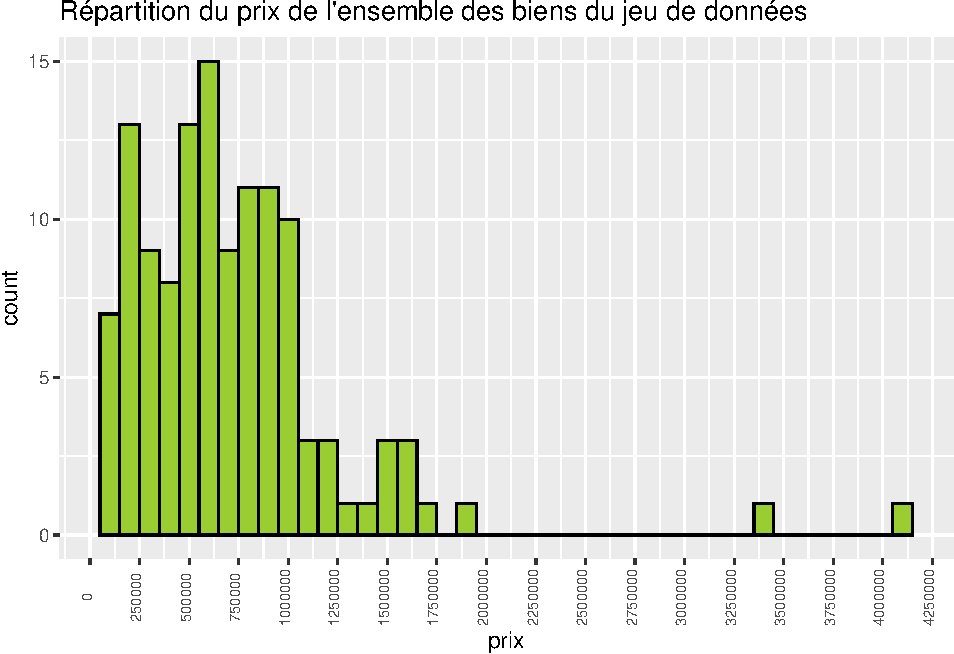
\includegraphics{Projet_files/figure-latex/unnamed-chunk-21-1.pdf}

\hypertarget{distance-des-biens-aux-stations}{%
\subsubsection{Distance des biens aux
stations}\label{distance-des-biens-aux-stations}}

Si on regarde les distances aux stations on remarque qu'en moyenne les
stations sont rangées dans l'ordre dans les annonces. Autrement dit, la
station la plus proche est nommer en premier dans l'annonce, suivi de la
deuxième station la plus proche pour finir par la troisième station de
métro/RER la plus proche. A noter que la distance Haversine est exprimée
en mètres et prend en compte l'ellipsoïde de la Terre. Cela n'a pas
vraiment d'incidence dans notre cas puisque les distances sont
relativement proche. Pour les distances des bies aux monuments par
exemple cela varie de simplement quelques mètres lorsqu'on prend en
compte ou non la sphère de la Terre. On remarque qu'en moyenne la
première station renseignée est à 228.03m du bien. 25\% des biens ont la
première station à moins de 152.25m. On constate également une répartion
plutôt équitablement répartie avec 50\% des biens ayant la première
station à moins de 229.32m et 50\% des autres ayant une station comprise
entre 229.32m et 539.63m. Pour ce qui est de la deuxième et troisième
station ont obtient également des répartions équitables puisqu'on a 50\%
des biens à moins de 387.49m de la station (maximum à 869.20m) dans le
premier cas, et 50\% des biens à moins de 490.3m de la station (maximum
à 1138.5m) dans le second cas. On peut ainsi confirmer que le nombre
important de stations de métros/RER dans Paris rend des distances
faibles puisque pratiquement tous les biens ont une station de métro/RER
à moins de 1km.

\begin{Shaded}
\begin{Highlighting}[]
\CommentTok{# Résumé statistique}

\KeywordTok{summary}\NormalTok{(biens_stat_des[,}\KeywordTok{c}\NormalTok{(}\DecValTok{10}\NormalTok{,}\DecValTok{11}\NormalTok{,}\DecValTok{12}\NormalTok{)])}
\end{Highlighting}
\end{Shaded}

\begin{verbatim}
##  distance_station_0 distance_station_1 distance_station_2
##  Min.   : 14.37     Min.   : 70.54     Min.   : 248.3    
##  1st Qu.:152.25     1st Qu.:315.16     1st Qu.: 403.4    
##  Median :229.32     Median :387.49     Median : 490.3    
##  Mean   :228.03     Mean   :415.35     Mean   : 534.9    
##  3rd Qu.:278.32     3rd Qu.:510.29     3rd Qu.: 635.5    
##  Max.   :539.63     Max.   :869.20     Max.   :1138.5
\end{verbatim}

\begin{Shaded}
\begin{Highlighting}[]
\CommentTok{# Représentation de la répartion des distances selon les stations}
\KeywordTok{par}\NormalTok{(}\DataTypeTok{xaxt=}\StringTok{"n"}\NormalTok{)}
\KeywordTok{boxplot}\NormalTok{(biens_stat_des}\OperatorTok{$}\NormalTok{distance_station_}\DecValTok{0}\NormalTok{,biens_stat_des}\OperatorTok{$}\NormalTok{distance_station_}\DecValTok{1}\NormalTok{,biens_stat_des}\OperatorTok{$}\NormalTok{distance_station_}\DecValTok{2}\NormalTok{,}\DataTypeTok{col=}\StringTok{"olivedrab3"}\NormalTok{,}\DataTypeTok{main=}\StringTok{"Représentation de la répartion des distances selon les stations"}\NormalTok{)}


\KeywordTok{axis}\NormalTok{(}\DecValTok{1}\NormalTok{, }\DataTypeTok{at=}\KeywordTok{seq}\NormalTok{(}\DecValTok{1}\NormalTok{, }\DecValTok{3}\NormalTok{, }\DataTypeTok{by=}\DecValTok{1}\NormalTok{), }\DataTypeTok{labels =} \OtherTok{FALSE}\NormalTok{,}\DataTypeTok{las=}\DecValTok{2}\NormalTok{)}
\KeywordTok{text}\NormalTok{(}\KeywordTok{seq}\NormalTok{(}\DecValTok{1}\NormalTok{, }\DecValTok{3}\NormalTok{, }\DataTypeTok{by=}\DecValTok{1}\NormalTok{), }\KeywordTok{par}\NormalTok{(}\StringTok{"usr"}\NormalTok{)[}\DecValTok{3}\NormalTok{] }\OperatorTok{-}\StringTok{ }\FloatTok{0.2}\NormalTok{, }\DataTypeTok{labels =} \KeywordTok{colnames}\NormalTok{(biens_stat_des[,}\KeywordTok{c}\NormalTok{(}\DecValTok{10}\NormalTok{,}\DecValTok{11}\NormalTok{,}\DecValTok{12}\NormalTok{)]),}\DataTypeTok{adj=} \FloatTok{1.1}\NormalTok{, }\DataTypeTok{srt =} \DecValTok{45}\NormalTok{, }\DataTypeTok{xpd =} \OtherTok{TRUE}\NormalTok{,}\DataTypeTok{cex=}\FloatTok{0.5}\NormalTok{)}
\end{Highlighting}
\end{Shaded}

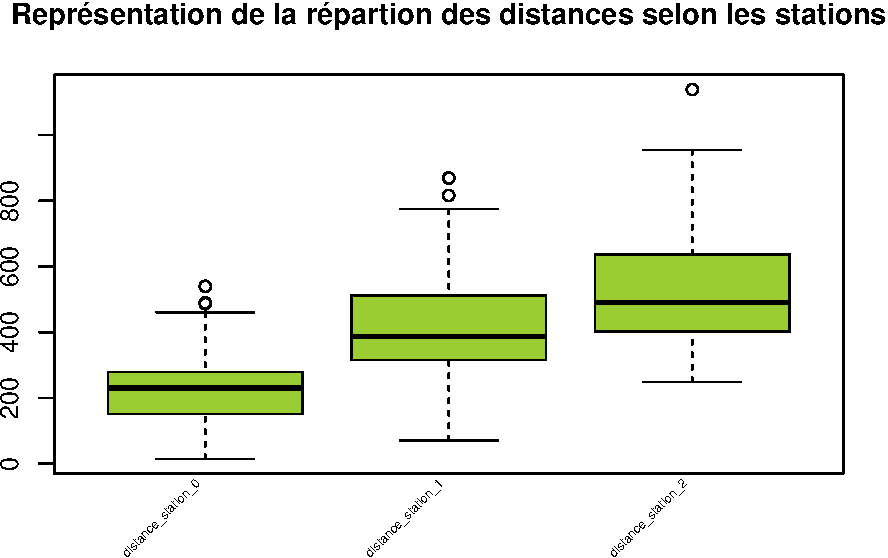
\includegraphics{Projet_files/figure-latex/unnamed-chunk-22-1.pdf}

\hypertarget{distance-des-biens-aux-monuments}{%
\subsubsection{Distance des biens aux
monuments}\label{distance-des-biens-aux-monuments}}

Si on regarde les distances des biens aux monuments les plus visités de
Paris on remarque qu'en moyenne tous nos biens sont plus proches du
Musée du Louvre, ils sont en moyenne à 3415.7m. On remarque que la Cité
des sciences et de l'industrie possède une distribution très étaléa
allant d'environ 500m à plus de 10km. Le fait est que ce monument est à
l'extrémité nord-est de Paris et donc un bien à l'extrémité sud-ouest
est à plus de 10km du monument.

\begin{Shaded}
\begin{Highlighting}[]
\CommentTok{# Résumé statistique}

\KeywordTok{summary}\NormalTok{(biens_stat_des[,}\KeywordTok{c}\NormalTok{(}\DecValTok{13}\NormalTok{,}\DecValTok{14}\NormalTok{,}\DecValTok{15}\NormalTok{,}\DecValTok{16}\NormalTok{,}\DecValTok{17}\NormalTok{,}\DecValTok{18}\NormalTok{,}\DecValTok{19}\NormalTok{,}\DecValTok{20}\NormalTok{,}\DecValTok{21}\NormalTok{,}\DecValTok{22}\NormalTok{,}\DecValTok{23}\NormalTok{)])}
\end{Highlighting}
\end{Shaded}

\begin{verbatim}
##  Cathédrale Notre-Dame de Paris Basilique du Sacré-Cœur de Montmartre
##  Min.   : 489.1                 Min.   : 403.4                       
##  1st Qu.:2565.8                 1st Qu.:2355.5                       
##  Median :3720.9                 Median :4324.0                       
##  Mean   :3623.1                 Mean   :4168.5                       
##  3rd Qu.:4644.3                 3rd Qu.:5943.1                       
##  Max.   :6951.4                 Max.   :8224.4                       
##  Musée du Louvre   Tour Eiffel     Centre Pompidou  Musée d’Orsay   
##  Min.   : 458.5   Min.   : 460.5   Min.   : 615.3   Min.   : 490.3  
##  1st Qu.:2543.3   1st Qu.:2439.6   1st Qu.:2329.2   1st Qu.:2623.7  
##  Median :3489.6   Median :4101.6   Median :3668.3   Median :3383.7  
##  Mean   :3415.7   Mean   :4325.9   Mean   :3520.1   Mean   :3495.0  
##  3rd Qu.:4274.6   3rd Qu.:5953.8   3rd Qu.:4320.4   3rd Qu.:4326.2  
##  Max.   :6394.3   Max.   :8596.4   Max.   :7360.5   Max.   :6339.9  
##  Cité des sciences et de l’industrie
##  Min.   :  803.3                    
##  1st Qu.: 4126.9                    
##  Median : 5854.1                    
##  Mean   : 5991.3                    
##  3rd Qu.: 7890.6                    
##  Max.   :11458.3                    
##  Chapelle Notre-Dame de la Médaille miraculeuse
##  Min.   : 562.3                                
##  1st Qu.:2697.2                                
##  Median :3775.5                                
##  Mean   :3699.0                                
##  3rd Qu.:4519.3                                
##  Max.   :6787.9                                
##  Grand site du Jardin des plantes Arc de triomphe   Grand Palais   
##  Min.   :  92.22                  Min.   : 542.7   Min.   : 268.1  
##  1st Qu.:2645.93                  1st Qu.:3146.8   1st Qu.:2461.0  
##  Median :3946.69                  Median :4217.3   Median :3602.9  
##  Mean   :3875.11                  Mean   :4466.5   Mean   :3754.1  
##  3rd Qu.:5110.92                  3rd Qu.:6302.6   3rd Qu.:4963.6  
##  Max.   :7044.63                  Max.   :9105.0   Max.   :7594.0
\end{verbatim}

\begin{Shaded}
\begin{Highlighting}[]
\CommentTok{# Représentation de la répartition des distances selon les monuments de Paris}

\KeywordTok{par}\NormalTok{(}\DataTypeTok{xaxt=}\StringTok{"n"}\NormalTok{)}
\KeywordTok{boxplot}\NormalTok{(biens_stat_des}\OperatorTok{$}\StringTok{`}\DataTypeTok{Cathédrale Notre-Dame de Paris}\StringTok{`}\NormalTok{,biens_stat_des}\OperatorTok{$}\StringTok{`}\DataTypeTok{Basilique du Sacré-Cœur de Montmartre}\StringTok{`}\NormalTok{,biens_stat_des}\OperatorTok{$}\StringTok{`}\DataTypeTok{Musée du Louvre}\StringTok{`}\NormalTok{,biens_stat_des}\OperatorTok{$}\StringTok{`}\DataTypeTok{Tour Eiffel}\StringTok{`}\NormalTok{,biens_stat_des}\OperatorTok{$}\StringTok{`}\DataTypeTok{Centre Pompidou}\StringTok{`}\NormalTok{,biens_stat_des}\OperatorTok{$}\StringTok{`}\DataTypeTok{Musée d’Orsay}\StringTok{`}\NormalTok{,biens_stat_des}\OperatorTok{$}\StringTok{`}\DataTypeTok{Cité des sciences et de l’industrie}\StringTok{`}\NormalTok{,biens_stat_des}\OperatorTok{$}\StringTok{`}\DataTypeTok{Chapelle Notre-Dame de la Médaille miraculeuse}\StringTok{`}\NormalTok{,biens_stat_des}\OperatorTok{$}\StringTok{`}\DataTypeTok{Grand site du Jardin des plantes}\StringTok{`}\NormalTok{,biens_stat_des}\OperatorTok{$}\StringTok{`}\DataTypeTok{Arc de triomphe}\StringTok{`}\NormalTok{,biens_stat_des}\OperatorTok{$}\StringTok{`}\DataTypeTok{Grand Palais}\StringTok{`}\NormalTok{,}\DataTypeTok{col=}\StringTok{"olivedrab3"}\NormalTok{,}\DataTypeTok{main=}\StringTok{"Représentation de la répartition des distances selon les monuments de Paris"}\NormalTok{,}\DataTypeTok{cex.main =} \FloatTok{0.9}\NormalTok{)}

\KeywordTok{axis}\NormalTok{(}\DecValTok{1}\NormalTok{, }\DataTypeTok{at=}\KeywordTok{seq}\NormalTok{(}\DecValTok{1}\NormalTok{, }\DecValTok{11}\NormalTok{, }\DataTypeTok{by=}\DecValTok{1}\NormalTok{), }\DataTypeTok{labels =} \OtherTok{FALSE}\NormalTok{,}\DataTypeTok{las=}\DecValTok{2}\NormalTok{)}
\KeywordTok{text}\NormalTok{(}\KeywordTok{seq}\NormalTok{(}\DecValTok{1}\NormalTok{, }\DecValTok{11}\NormalTok{, }\DataTypeTok{by=}\DecValTok{1}\NormalTok{), }\KeywordTok{par}\NormalTok{(}\StringTok{"usr"}\NormalTok{)[}\DecValTok{3}\NormalTok{] }\OperatorTok{-}\StringTok{ }\FloatTok{0.2}\NormalTok{, }\DataTypeTok{labels =} \KeywordTok{colnames}\NormalTok{(biens_stat_des[,}\KeywordTok{c}\NormalTok{(}\DecValTok{13}\NormalTok{,}\DecValTok{14}\NormalTok{,}\DecValTok{15}\NormalTok{,}\DecValTok{16}\NormalTok{,}\DecValTok{17}\NormalTok{,}\DecValTok{18}\NormalTok{,}\DecValTok{19}\NormalTok{,}\DecValTok{20}\NormalTok{,}\DecValTok{21}\NormalTok{,}\DecValTok{22}\NormalTok{,}\DecValTok{23}\NormalTok{)]),}\DataTypeTok{adj=} \FloatTok{1.1}\NormalTok{, }\DataTypeTok{srt =} \DecValTok{45}\NormalTok{, }\DataTypeTok{xpd =} \OtherTok{TRUE}\NormalTok{,}\DataTypeTok{cex=}\FloatTok{0.5}\NormalTok{)}
\end{Highlighting}
\end{Shaded}

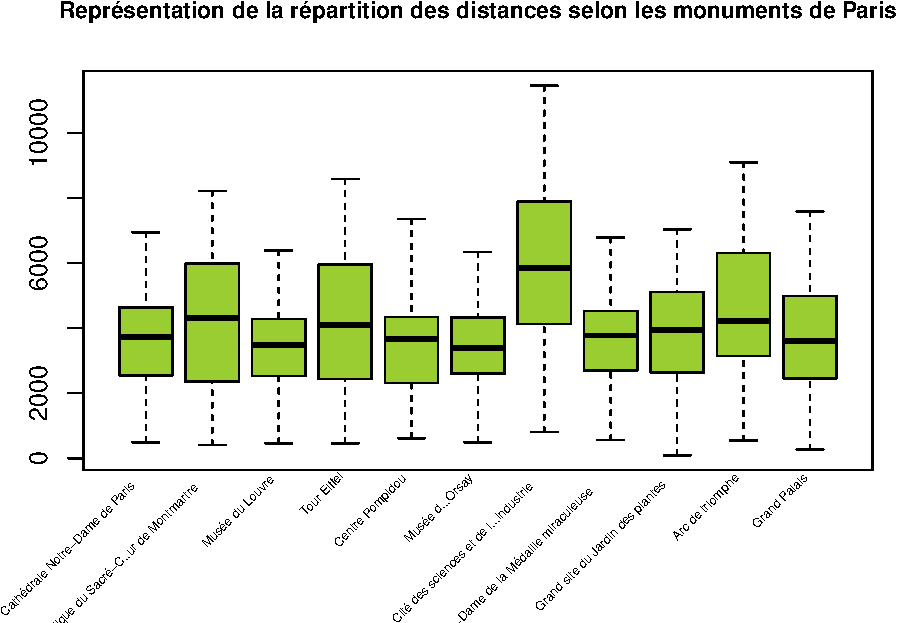
\includegraphics{Projet_files/figure-latex/unnamed-chunk-23-1.pdf}
\#\#\# Prix des biens en fonction de la zone géographique dans Paris

On remarque que le fait que les biens soient dans l'hyper-centre ou non
de Paris n'a pas d'influence sur les prix. Les deux médianes sont autour
de 600000euros avec une concentration légèrement plus forte pour les
biens dans les arrondissement périphériques de Paris (i. e. du 12e au
20e)

\begin{Shaded}
\begin{Highlighting}[]
\CommentTok{# Répartition du prix des biens en fonction de la zone géographique}

\KeywordTok{boxplot}\NormalTok{(biens_stat_des}\OperatorTok{$}\NormalTok{prix}\OperatorTok{~}\NormalTok{biens_stat_des}\OperatorTok{$}\NormalTok{arrondissement,}\DataTypeTok{names=}\KeywordTok{c}\NormalTok{(}\StringTok{"Arrondissement hyper-centre"}\NormalTok{,}\StringTok{"Arrondissement périphérie"}\NormalTok{),}\DataTypeTok{col=}\StringTok{"olivedrab3"}\NormalTok{,}\DataTypeTok{ylab=}\StringTok{"prix des biens"}\NormalTok{,}\DataTypeTok{main=}\StringTok{"Répartition du prix des biens selon la zone géographique"}\NormalTok{,}\DataTypeTok{ylim=}\KeywordTok{c}\NormalTok{(}\DecValTok{0}\NormalTok{,}\DecValTok{2000000}\NormalTok{))}
\end{Highlighting}
\end{Shaded}

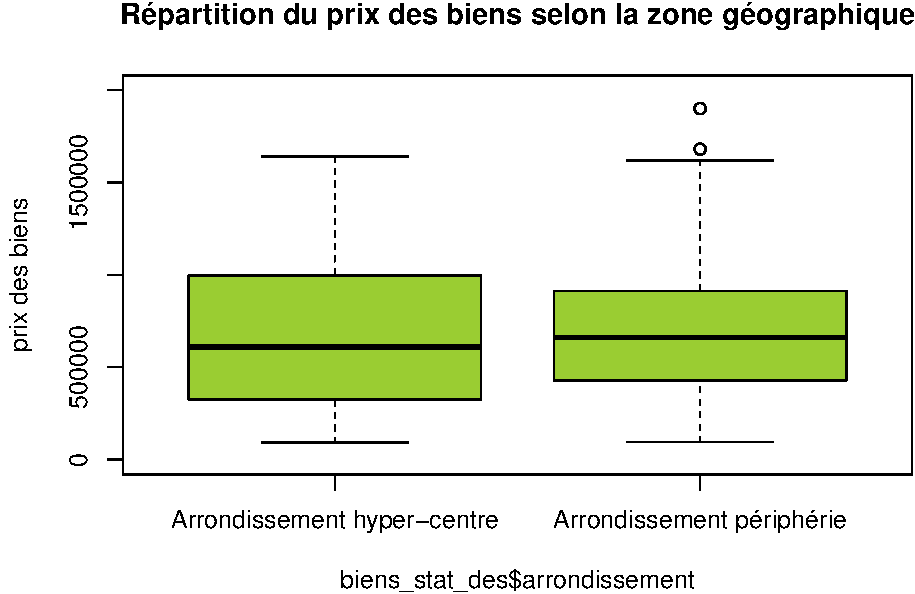
\includegraphics{Projet_files/figure-latex/unnamed-chunk-24-1.pdf}

\hypertarget{prix-des-biens-en-fonction-du-type-de-biens}{%
\subsubsection{Prix des biens en fonction du type de
biens}\label{prix-des-biens-en-fonction-du-type-de-biens}}

On a choisit de séparer les biens selon leur type pour essayer de mettre
en évidence le répartition du prix selon le type de bien. On remarque
que le prix des maisons est nettement supérieur au prix des appartement,
75\% des maisons (3 en réalité\ldots{}) ont un prix supérieur à
pratiquement 100\% des appartement lorsqu'on se place au prix de
1500000euros.

\begin{Shaded}
\begin{Highlighting}[]
\CommentTok{#Répartition du prix des bien en fonction de tous les types de biens}

\NormalTok{rep_biens <-}\StringTok{ }\KeywordTok{ggplot}\NormalTok{(}\DataTypeTok{data=}\NormalTok{biens, }\KeywordTok{aes}\NormalTok{(}\DataTypeTok{x=}\NormalTok{type, }\DataTypeTok{y=}\NormalTok{prix,}\DataTypeTok{fill=}\NormalTok{type))}
\NormalTok{rep_biens <-}\StringTok{ }\NormalTok{rep_biens }\OperatorTok{+}\KeywordTok{ggtitle}\NormalTok{(}\StringTok{"Répartition du prix des biens en fonction du type de bien"}\NormalTok{)}\OperatorTok{+}\StringTok{ }\KeywordTok{geom_boxplot}\NormalTok{()}\OperatorTok{+}\StringTok{ }\KeywordTok{scale_y_continuous}\NormalTok{(}\DataTypeTok{name=}\StringTok{"prix des biens"}\NormalTok{)}\OperatorTok{+}\StringTok{ }\KeywordTok{theme}\NormalTok{(}\DataTypeTok{axis.text.x =} \KeywordTok{element_blank}\NormalTok{())}
\NormalTok{rep_biens}
\end{Highlighting}
\end{Shaded}

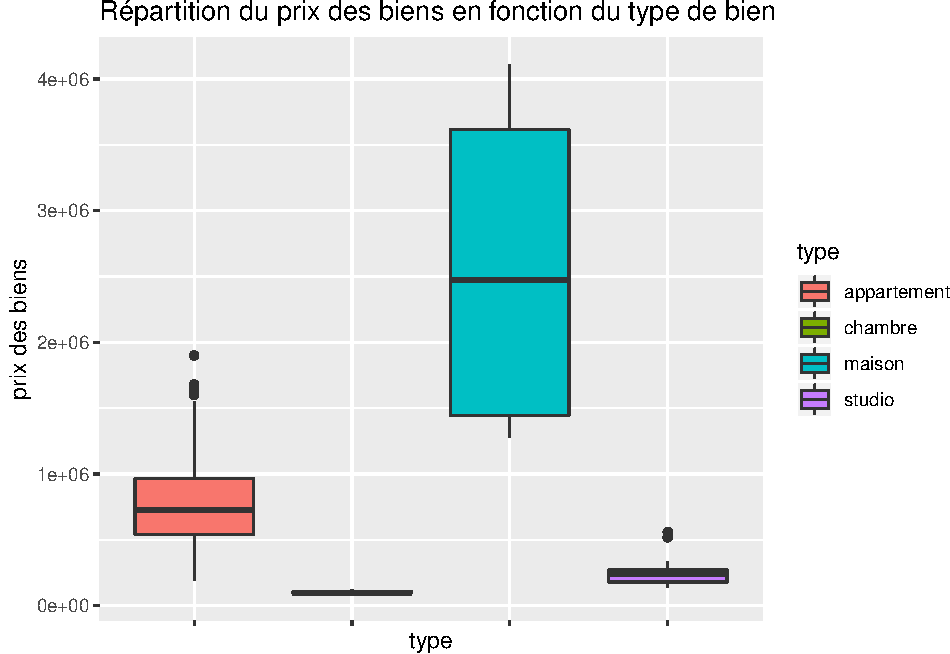
\includegraphics{Projet_files/figure-latex/unnamed-chunk-25-1.pdf}

On a choisit de supprimer les maisons dans la représentation suivante
pour limiter l'écrasement des répartitions des prix des chambres et
studio. On constate que 100\% des chambres sont moins chères que les
studio et appartements. Une chambre est associée à l'absence d'une
cuisine, WC et douches dans le logement. On remarque aussi que le prix
des appartements varie de 250000euros à plus de 1500000euros (soit plus
6 fois son prix minimum qui est pourtant élevé\ldots{}) avec un prix
médian à 750000euros selon notre jeu de données. Le prix médian d'un
studio est de 250000euros à Paris selon notre jeu de données.

\begin{Shaded}
\begin{Highlighting}[]
\CommentTok{# On élimine les maisons pour voir plus en détails la répartition des autres type de biens}

\NormalTok{biens_sans_mai<-biens[}\KeywordTok{order}\NormalTok{(biens}\OperatorTok{$}\NormalTok{type),][}\OperatorTok{-}\KeywordTok{c}\NormalTok{(}\DecValTok{100}\NormalTok{,}\DecValTok{101}\NormalTok{,}\DecValTok{102}\NormalTok{,}\DecValTok{103}\NormalTok{),]}


\CommentTok{# On obtient une nouvelle représentation}

\NormalTok{rep_biens_sans_mai <-}\StringTok{ }\KeywordTok{ggplot}\NormalTok{(}\DataTypeTok{data=}\NormalTok{biens_sans_mai, }\KeywordTok{aes}\NormalTok{(}\DataTypeTok{x=}\NormalTok{type, }\DataTypeTok{y=}\NormalTok{prix,}\DataTypeTok{fill=}\NormalTok{type))}
\NormalTok{rep_biens_sans_mai<-}\StringTok{ }\NormalTok{rep_biens_sans_mai }\OperatorTok{+}\KeywordTok{ggtitle}\NormalTok{(}\StringTok{"Répartition du prix d'un bien en fonction du type de bien (sans maison)"}\NormalTok{)}\OperatorTok{+}\KeywordTok{geom_boxplot}\NormalTok{()}\OperatorTok{+}\StringTok{ }\KeywordTok{scale_y_continuous}\NormalTok{(}\DataTypeTok{name=}\StringTok{"prix des biens"}\NormalTok{)}\OperatorTok{+}\StringTok{ }\KeywordTok{theme}\NormalTok{(}\DataTypeTok{axis.text.x =} \KeywordTok{element_blank}\NormalTok{())}
\NormalTok{rep_biens_sans_mai}
\end{Highlighting}
\end{Shaded}

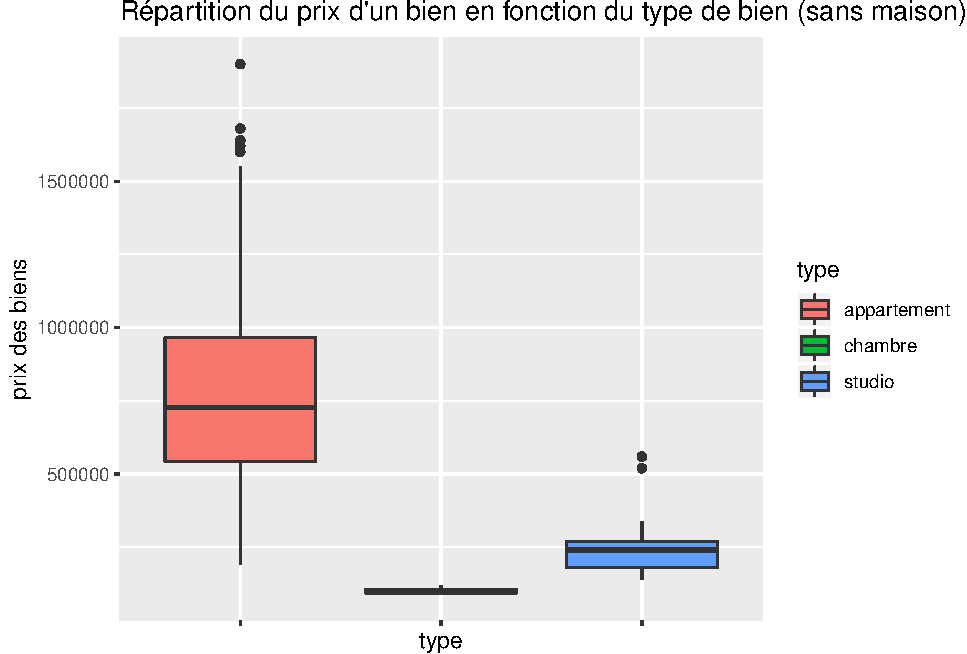
\includegraphics{Projet_files/figure-latex/unnamed-chunk-26-1.pdf}

On a choisit d'effectuer une régression du prix des biens en fonction de
la surface et du type de bien. Les données sont intéressantes à analyser
puisqu'on constate avec notre jeu de données que le prix d'une maison de
75m2 équivaut à celui d'un appartement de 75m2. Cependant, toutes les
analyses ne sont pas correctes. Il serait faux de dire que le prix d'une
chambre de 50m2 équivaut au prix d'une maison de 50m2 puisque par
définition une chambre en vente dépasse rarement les 15m2 dans Paris.
Pourtant, c'est ce que nous dit ce graphique. Pour finir, on remarque
que la surface à plus d'incidence sur le prix d'une maison que sur le
prix d'un bien, autrement dit 1m2 en plus va faire augmenter plus
fortement le prix d'une maison que le prix d'un appartement.

\begin{Shaded}
\begin{Highlighting}[]
\CommentTok{# régression du prix des biens en fonction du type de bien}

\KeywordTok{ggplot}\NormalTok{(biens,}\KeywordTok{aes}\NormalTok{(}\DataTypeTok{x=}\NormalTok{surface,}\DataTypeTok{y=}\NormalTok{prix,}\DataTypeTok{color=}\NormalTok{type, }\DataTypeTok{shape=}\NormalTok{type))}\OperatorTok{+}\KeywordTok{geom_point}\NormalTok{() }\OperatorTok{+}\KeywordTok{scale_y_continuous}\NormalTok{(}\DataTypeTok{name=}\StringTok{"prix des biens"}\NormalTok{)}\OperatorTok{+}\KeywordTok{ggtitle}\NormalTok{(}\StringTok{"Evolution du prix du bien en fonction de la surface pour chaque type de bien"}\NormalTok{)}\OperatorTok{+}\KeywordTok{scale_x_continuous}\NormalTok{(}\DataTypeTok{name=}\StringTok{"surface des biens en m2"}\NormalTok{, }\DataTypeTok{limits=}\KeywordTok{c}\NormalTok{(}\DecValTok{0}\NormalTok{, }\DecValTok{260}\NormalTok{))}\OperatorTok{+}\StringTok{ }\KeywordTok{geom_smooth}\NormalTok{(}\DataTypeTok{method=}\NormalTok{lm, }\DataTypeTok{se=}\OtherTok{FALSE}\NormalTok{,}\DataTypeTok{fullrange=}\OtherTok{TRUE}\NormalTok{)}
\end{Highlighting}
\end{Shaded}

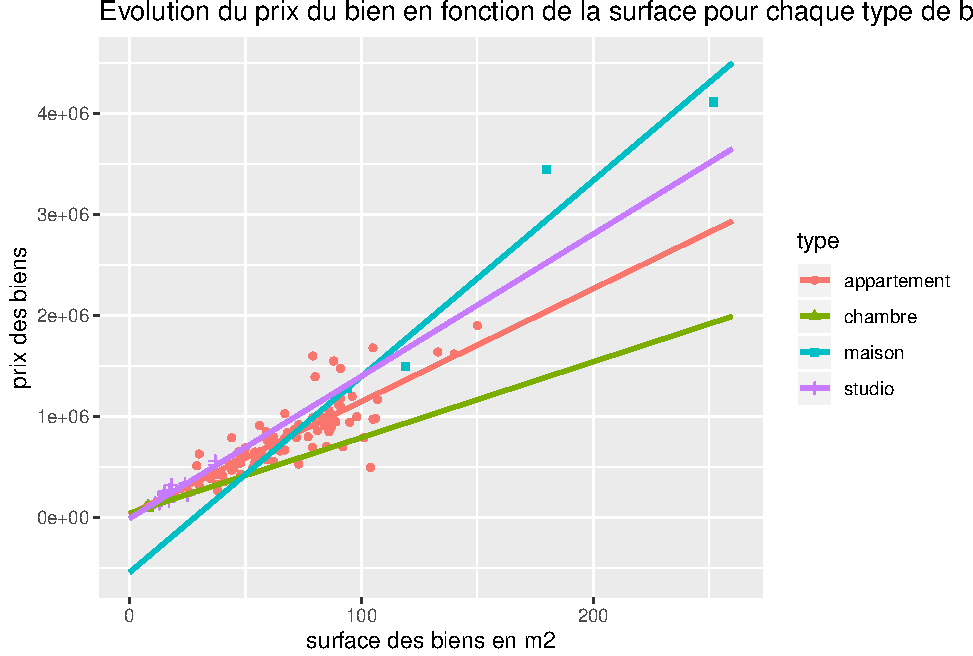
\includegraphics{Projet_files/figure-latex/unnamed-chunk-27-1.pdf}

\hypertarget{matrice-de-variance-covariance}{%
\subsubsection{Matrice de
variance-covariance}\label{matrice-de-variance-covariance}}

La matrice de variance-covariance nous sert à sélectionner dans notre
modèle final que les variables indépendantes entre-elles. Sans surprise,
on remarque que la surface d'un bien est fortement corrélé avec le
nombre de pièces et le nombre de chambre. A l'aide de cette matrice nous
remarquons également que les monuments proches sont fortement corrélés
entre eux. Par exemple, le centre Pompidou et Cathédrale Notre-Dame de
Paris ont une covariance de 0.94. Lorsqu'on sélectionnera le modèle
final il faudra s'assurer que nous avons pas garder des monuments
proches pour avoir des variables décorrélées entre elles.

\begin{Shaded}
\begin{Highlighting}[]
\NormalTok{mat_cor <-}\StringTok{ }\KeywordTok{round}\NormalTok{(}\KeywordTok{cor}\NormalTok{(biens[,}\KeywordTok{c}\NormalTok{(}\DecValTok{6}\NormalTok{,}\DecValTok{12}\NormalTok{,}\DecValTok{13}\NormalTok{,}\DecValTok{14}\NormalTok{,}\DecValTok{24}\NormalTok{,}\DecValTok{25}\NormalTok{,}\DecValTok{26}\NormalTok{,}\DecValTok{27}\NormalTok{,}\DecValTok{28}\NormalTok{,}\DecValTok{29}\NormalTok{,}\DecValTok{30}\NormalTok{,}\DecValTok{31}\NormalTok{,}\DecValTok{32}\NormalTok{,}\DecValTok{33}\NormalTok{,}\DecValTok{34}\NormalTok{,}\DecValTok{35}\NormalTok{,}\DecValTok{36}\NormalTok{,}\DecValTok{37}\NormalTok{,}\DecValTok{38}\NormalTok{)]),}\DecValTok{2}\NormalTok{)}
\KeywordTok{rownames}\NormalTok{(mat_cor) <-}\StringTok{ }\KeywordTok{colnames}\NormalTok{(biens[,}\KeywordTok{c}\NormalTok{(}\DecValTok{6}\NormalTok{,}\DecValTok{12}\NormalTok{,}\DecValTok{13}\NormalTok{,}\DecValTok{14}\NormalTok{,}\DecValTok{24}\NormalTok{,}\DecValTok{25}\NormalTok{,}\DecValTok{26}\NormalTok{,}\DecValTok{27}\NormalTok{,}\DecValTok{28}\NormalTok{,}\DecValTok{29}\NormalTok{,}\DecValTok{30}\NormalTok{,}\DecValTok{31}\NormalTok{,}\DecValTok{32}\NormalTok{,}\DecValTok{33}\NormalTok{,}\DecValTok{34}\NormalTok{,}\DecValTok{35}\NormalTok{,}\DecValTok{36}\NormalTok{,}\DecValTok{37}\NormalTok{,}\DecValTok{38}\NormalTok{)])}

\KeywordTok{colnames}\NormalTok{(mat_cor) <-}\KeywordTok{colnames}\NormalTok{(biens[,}\KeywordTok{c}\NormalTok{(}\DecValTok{6}\NormalTok{,}\DecValTok{12}\NormalTok{,}\DecValTok{13}\NormalTok{,}\DecValTok{14}\NormalTok{,}\DecValTok{24}\NormalTok{,}\DecValTok{25}\NormalTok{,}\DecValTok{26}\NormalTok{,}\DecValTok{27}\NormalTok{,}\DecValTok{28}\NormalTok{,}\DecValTok{29}\NormalTok{,}\DecValTok{30}\NormalTok{,}\DecValTok{31}\NormalTok{,}\DecValTok{32}\NormalTok{,}\DecValTok{33}\NormalTok{,}\DecValTok{34}\NormalTok{,}\DecValTok{35}\NormalTok{,}\DecValTok{36}\NormalTok{,}\DecValTok{37}\NormalTok{,}\DecValTok{38}\NormalTok{)])}

\NormalTok{mat_cor<-}\KeywordTok{data.frame}\NormalTok{(mat_cor)}
\KeywordTok{head}\NormalTok{(mat_cor)}
\end{Highlighting}
\end{Shaded}

\begin{verbatim}
##                    nb_photo nb_pieces nb_chambres surface distance_station_0
## nb_photo               1.00      0.21        0.23    0.22               0.05
## nb_pieces              0.21      1.00        0.94    0.91               0.15
## nb_chambres            0.23      0.94        1.00    0.84               0.17
## surface                0.22      0.91        0.84    1.00               0.09
## distance_station_0     0.05      0.15        0.17    0.09               1.00
## distance_station_1     0.08      0.24        0.26    0.21               0.31
##                    distance_station_1 distance_station_2
## nb_photo                         0.08               0.01
## nb_pieces                        0.24              -0.05
## nb_chambres                      0.26              -0.03
## surface                          0.21              -0.05
## distance_station_0               0.31               0.25
## distance_station_1               1.00               0.35
##                    Cathédrale.Notre.Dame.de.Paris
## nb_photo                                     0.12
## nb_pieces                                    0.18
## nb_chambres                                  0.23
## surface                                      0.17
## distance_station_0                           0.10
## distance_station_1                           0.18
##                    Basilique.du.Sacré.Cœur.de.Montmartre Musée.du.Louvre
## nb_photo                                            0.08            0.11
## nb_pieces                                           0.29            0.27
## nb_chambres                                         0.32            0.32
## surface                                             0.25            0.20
## distance_station_0                                  0.12            0.14
## distance_station_1                                  0.12            0.26
##                    Tour.Eiffel Centre.Pompidou Musée.d.Orsay
## nb_photo                 -0.02            0.12          0.08
## nb_pieces                 0.10            0.23          0.23
## nb_chambres               0.10            0.28          0.28
## surface                  -0.01            0.22          0.13
## distance_station_0        0.03            0.13          0.12
## distance_station_1        0.11            0.18          0.26
##                    Cité.des.sciences.et.de.l.industrie
## nb_photo                                          0.06
## nb_pieces                                         0.16
## nb_chambres                                       0.18
## surface                                           0.20
## distance_station_0                                0.08
## distance_station_1                                0.02
##                    Chapelle.Notre.Dame.de.la.Médaille.miraculeuse
## nb_photo                                                     0.04
## nb_pieces                                                    0.13
## nb_chambres                                                  0.16
## surface                                                      0.05
## distance_station_0                                           0.04
## distance_station_1                                           0.20
##                    Grand.site.du.Jardin.des.plantes Arc.de.triomphe
## nb_photo                                       0.11            0.00
## nb_pieces                                      0.11            0.18
## nb_chambres                                    0.14            0.20
## surface                                        0.12            0.05
## distance_station_0                             0.06            0.06
## distance_station_1                             0.13            0.14
##                    Grand.Palais distance_université_plus_près
## nb_photo                   0.03                          0.01
## nb_pieces                  0.21                          0.03
## nb_chambres                0.24                          0.05
## surface                    0.08                         -0.09
## distance_station_0         0.09                          0.05
## distance_station_1         0.20                          0.04
\end{verbatim}

\hypertarget{moduxe8les-economuxe9trique}{%
\section{Modèles Econométrique}\label{moduxe8les-economuxe9trique}}

\hypertarget{construction-du-moduxe8le-optimal.}{%
\subsection{Construction du Modèle
``Optimal''.}\label{construction-du-moduxe8le-optimal.}}

Durant cette partie nous utiliserons le
\texttt{data.frame\ biens\_stat\_des}

Extrayons dans un premier temps notre Y et notre X: le prix d'un bien
(Y) et Les variables exogènes (X) en prenant soin de retirer la variable
maison (par soucis du rang de la matrice de design).

\hypertarget{premier-moduxe8le-nauxeff}{%
\subsubsection{Premier modèle
``Naïf''}\label{premier-moduxe8le-nauxeff}}

Nous crééons un premier modèle avec toutes les variables explicatives.

\begin{Shaded}
\begin{Highlighting}[]
\NormalTok{lm_}\DecValTok{1}\NormalTok{=}\KeywordTok{lm}\NormalTok{(Y}\OperatorTok{~}\NormalTok{.,}\DataTypeTok{data=}\NormalTok{X)  }
\KeywordTok{summary}\NormalTok{(lm_}\DecValTok{1}\NormalTok{)}
\end{Highlighting}
\end{Shaded}

\begin{verbatim}
## 
## Call:
## lm(formula = Y ~ ., data = X)
## 
## Residuals:
##     Min      1Q  Median      3Q     Max 
## -597981  -56713     216   60918  709974 
## 
## Coefficients:
##                                                    Estimate Std. Error t value
## (Intercept)                                       3.593e+05  2.916e+05   1.232
## appartement                                      -4.702e+05  1.187e+05  -3.961
## studio                                           -4.259e+05  1.438e+05  -2.961
## chambre                                          -4.698e+05  1.611e+05  -2.917
## nb_photo                                          2.352e+03  4.250e+03   0.553
## nb_pieces                                        -7.815e+04  4.668e+04  -1.674
## nb_chambres                                       3.930e+04  4.561e+04   0.862
## surface                                           1.394e+04  1.164e+03  11.975
## distance_station_0                                1.235e+01  1.511e+02   0.082
## distance_station_1                               -1.640e+01  1.277e+02  -0.128
## distance_station_2                               -1.383e+02  1.065e+02  -1.299
## `Cathédrale Notre-Dame de Paris`                 -2.686e+02  3.936e+02  -0.682
## `Basilique du Sacré-Cœur de Montmartre`           2.365e+00  4.309e+01   0.055
## `Musée du Louvre`                                 1.044e+03  3.715e+02   2.809
## `Tour Eiffel`                                    -5.735e+01  7.395e+01  -0.775
## `Centre Pompidou`                                -8.073e+01  1.950e+02  -0.414
## `Musée d’Orsay`                                  -1.870e+03  5.430e+02  -3.444
## `Cité des sciences et de l’industrie`             2.013e+01  3.327e+01   0.605
## `Chapelle Notre-Dame de la Médaille miraculeuse`  5.701e+02  1.935e+02   2.945
## `Grand site du Jardin des plantes`                1.424e+02  2.194e+02   0.649
## `Arc de triomphe`                                 2.482e+01  7.499e+01   0.331
## `Grand Palais`                                    4.776e+02  2.056e+02   2.323
## distance_université_plus_près                    -1.481e+01  3.567e+01  -0.415
## arrondissement                                    1.648e+04  6.360e+04   0.259
##                                                  Pr(>|t|)    
## (Intercept)                                      0.220662    
## appartement                                      0.000140 ***
## studio                                           0.003831 ** 
## chambre                                          0.004366 ** 
## nb_photo                                         0.581229    
## nb_pieces                                        0.097239 .  
## nb_chambres                                      0.390977    
## surface                                           < 2e-16 ***
## distance_station_0                               0.935013    
## distance_station_1                               0.898107    
## distance_station_2                               0.197026    
## `Cathédrale Notre-Dame de Paris`                 0.496566    
## `Basilique du Sacré-Cœur de Montmartre`          0.956341    
## `Musée du Louvre`                                0.005970 ** 
## `Tour Eiffel`                                    0.439881    
## `Centre Pompidou`                                0.679710    
## `Musée d’Orsay`                                  0.000839 ***
## `Cité des sciences et de l’industrie`            0.546473    
## `Chapelle Notre-Dame de la Médaille miraculeuse` 0.004012 ** 
## `Grand site du Jardin des plantes`               0.517733    
## `Arc de triomphe`                                0.741337    
## `Grand Palais`                                   0.022192 *  
## distance_université_plus_près                    0.678884    
## arrondissement                                   0.796075    
## ---
## Signif. codes:  0 '***' 0.001 '**' 0.01 '*' 0.05 '.' 0.1 ' ' 1
## 
## Residual standard error: 164400 on 100 degrees of freedom
## Multiple R-squared:  0.9284, Adjusted R-squared:  0.912 
## F-statistic: 56.39 on 23 and 100 DF,  p-value: < 2.2e-16
\end{verbatim}

Nous pouvons noter que la variable la plus signicative est la
\texttt{surface}. Nous nous y attendions. Nous remarquons que les
variables \texttt{Chapelle\ Notre-Dame\ de\ la\ Médaille\ miraculeuse}
et \texttt{Musée\ d’Orsay} sont toutes deux significatives (au seuil de
5\%), elles correspondent aux distances à ces deux monuments qui se
trouvent dans le même arrondissement et tout deux plutôt au centre de
Paris. Ainsi nous pouvons allons créer 3 sous-modèles l'un avec la
moyenne des distance au monuments, un deuxième avec seulement
\texttt{Musée\ d’Orsay} et un dernier avec seulement
\texttt{Chapelle\ Notre-Dame\ de\ la\ Médaille\ miraculeuse} (toutes
spécifications/modification égales par ailleurs).

La présence d'une université proche
(\texttt{distance\_université\_plus\_près}) d'un bien ne semble pas
avoir d'impact significatif (au seuil de 5\%) sur le prix. Pareillement
pour \texttt{distance\_station\_0}. Nous remarquons aussi que les
variables \texttt{arrondissement} (qui décrit la zone,
\texttt{nb\_photo},\texttt{Centre\ Pompidou},\texttt{Cathédrale\ Notre-Dame\ de\ Paris},
\texttt{Cité\ des\ sciences\ et\ de\ l’industrie},
\texttt{Grand\ site\ du\ Jardin\ des\ plantes} et ne sont pas non plus
significatives (au seuil de 5\%).

De plus les variables \texttt{surface}, \texttt{nb\_pieces} et
\texttt{nb\_chambres} sont toutes les trois très corrélées positivements
et portent une certaine redondance d'information (en effet, un bien avec
une grande surface aura tendance à avoir plus de pièces et le nombre de
pièce contient déjà le nombre de chambre).\\
Ainsi nous prenons allons remplacer ces trois variables par le rapport
\(\frac{surface}{nb_piece}\).

\begin{Shaded}
\begin{Highlighting}[]
\CommentTok{# Création nouvelle variable Rapport}
\NormalTok{biens_stat_des=}\KeywordTok{cbind}\NormalTok{(biens_stat_des,}\DataTypeTok{Rapport=}\NormalTok{biens_stat_des}\OperatorTok{$}\NormalTok{surface}\OperatorTok{/}\NormalTok{biens_stat_des}\OperatorTok{$}\NormalTok{nb_pieces)}
\CommentTok{# Suppression de surface, nb_pieces, nb_chambres}
\NormalTok{biens_stat_des =}\StringTok{ }\KeywordTok{select}\NormalTok{(biens_stat_des, }\OperatorTok{-}\KeywordTok{c}\NormalTok{(surface,nb_pieces,nb_chambres))}
\end{Highlighting}
\end{Shaded}

\#Création des 3 datasets pour les 3 sous-modèles

\begin{Shaded}
\begin{Highlighting}[]
\CommentTok{## Dataset avec les moyennes ==> Ajout d'une variable Moyenne_ORSAY_CHAPELLE_var}
\NormalTok{Moyenne_ORSAY_CHAPELLE_var=}\KeywordTok{rowMeans}\NormalTok{(biens_stat_des[,}\KeywordTok{c}\NormalTok{(}\DecValTok{9}\NormalTok{,}\DecValTok{8}\NormalTok{)])}

\CommentTok{## Ajout au dataset adéquat: biens_stat_des_Moyenne}
\NormalTok{biens_stat_des_Moyenne=}\KeywordTok{cbind}\NormalTok{(biens_stat_des,}\DataTypeTok{Moyenne_ORSAY_CHAPELLE=}\NormalTok{Moyenne_ORSAY_CHAPELLE_var)}

\CommentTok{## Suppression des autres variables }
\NormalTok{biens_stat_des_Moyenne=}\KeywordTok{select}\NormalTok{(biens_stat_des_Moyenne,}\OperatorTok{-}\KeywordTok{c}\NormalTok{(}\StringTok{`}\DataTypeTok{Musée d’Orsay}\StringTok{`}\NormalTok{,}\StringTok{`}\DataTypeTok{Chapelle Notre-Dame de la Médaille miraculeuse}\StringTok{`}\NormalTok{))}
\end{Highlighting}
\end{Shaded}

\begin{Shaded}
\begin{Highlighting}[]
\CommentTok{## Dataset avec la distance au Musée d'Orsay ==> Suppression de Chapelle Notre-Dame de la Médaille miraculeuse}
\NormalTok{biens_stat_des_ORSAY=}\KeywordTok{select}\NormalTok{(biens_stat_des,}\OperatorTok{-}\KeywordTok{c}\NormalTok{(}\StringTok{`}\DataTypeTok{Chapelle Notre-Dame de la Médaille miraculeuse}\StringTok{`}\NormalTok{))}

\CommentTok{## Dataset avec la distance à la Chapelle Notre-Dame de la Médaille miraculeuse ==> Suppression de Musée d'Orsay }
\NormalTok{biens_stat_des_Chapelle=}\KeywordTok{select}\NormalTok{(biens_stat_des,}\OperatorTok{-}\KeywordTok{c}\NormalTok{(}\StringTok{`}\DataTypeTok{Musée d’Orsay}\StringTok{`}\NormalTok{))}
\end{Highlighting}
\end{Shaded}

\hypertarget{selection-du-meilleur-2uxe8me-moduxe8le}{%
\subsection{Selection du meilleur 2ème
Modèle}\label{selection-du-meilleur-2uxe8me-moduxe8le}}

\hypertarget{procuxe9dure}{%
\subsubsection{Procédure}\label{procuxe9dure}}

Nous allons donc fitter 3 sous-modèle et selectionner le sous-modèle
ayant la vairable la plus significative. \#\#\# Fit Sous-modèle 1 :
\texttt{Moyenne\_ORSAY\_CHAPELLE}

\begin{Shaded}
\begin{Highlighting}[]
\NormalTok{X=biens_stat_des_Moyenne}
\NormalTok{lm_}\DecValTok{2}\NormalTok{_}\DecValTok{1}\NormalTok{=}\KeywordTok{lm}\NormalTok{(Y}\OperatorTok{~}\NormalTok{.,}\DataTypeTok{data=}\NormalTok{X)  }
\KeywordTok{summary}\NormalTok{(lm_}\DecValTok{2}\NormalTok{_}\DecValTok{1}\NormalTok{)}
\end{Highlighting}
\end{Shaded}

\begin{verbatim}
## 
## Call:
## lm(formula = Y ~ ., data = X)
## 
## Residuals:
##      Min       1Q   Median       3Q      Max 
## -1185160  -146467    -5171   140384  1503281 
## 
## Coefficients:
##                          Estimate Std. Error t value Pr(>|t|)    
## (Intercept)             1.673e+06  2.891e+05   5.788 6.61e-08 ***
## appartement            -1.648e+06  1.728e+05  -9.540 3.81e-16 ***
## studio                 -2.036e+06  1.870e+05 -10.886  < 2e-16 ***
## chambre                -1.894e+06  2.373e+05  -7.983 1.36e-12 ***
## distance_station_1      1.765e+02  2.191e+02   0.806   0.4221    
## distance_station_2     -3.910e+02  1.839e+02  -2.126   0.0357 *  
## `Musée du Louvre`       1.421e+02  1.124e+02   1.265   0.2085    
## `Tour Eiffel`           2.218e+01  9.150e+01   0.242   0.8089    
## `Arc de triomphe`       1.480e+02  1.128e+02   1.312   0.1921    
## `Grand Palais`         -2.744e+02  1.776e+02  -1.545   0.1252    
## Rapport                 3.352e+04  5.312e+03   6.310 5.73e-09 ***
## Moyenne_ORSAY_CHAPELLE -1.738e+01  1.448e+02  -0.120   0.9047    
## ---
## Signif. codes:  0 '***' 0.001 '**' 0.01 '*' 0.05 '.' 0.1 ' ' 1
## 
## Residual standard error: 317400 on 112 degrees of freedom
## Multiple R-squared:  0.7012, Adjusted R-squared:  0.6718 
## F-statistic: 23.89 on 11 and 112 DF,  p-value: < 2.2e-16
\end{verbatim}

\hypertarget{fit-sous-moduxe8le-2-musuxe9e-dorsay}{%
\subsubsection{\texorpdfstring{Fit Sous-modèle 2 :
\texttt{Musée\ d\textquotesingle{}Orsay}}{Fit Sous-modèle 2 : Musée d'Orsay}}\label{fit-sous-moduxe8le-2-musuxe9e-dorsay}}

\begin{Shaded}
\begin{Highlighting}[]
\NormalTok{X=biens_stat_des_ORSAY}
\NormalTok{lm_}\DecValTok{2}\NormalTok{_}\DecValTok{2}\NormalTok{=}\KeywordTok{lm}\NormalTok{(Y}\OperatorTok{~}\NormalTok{.,}\DataTypeTok{data=}\NormalTok{X)  }
\KeywordTok{summary}\NormalTok{(lm_}\DecValTok{2}\NormalTok{_}\DecValTok{2}\NormalTok{)}
\end{Highlighting}
\end{Shaded}

\begin{verbatim}
## 
## Call:
## lm(formula = Y ~ ., data = X)
## 
## Residuals:
##      Min       1Q   Median       3Q      Max 
## -1149989  -151546   -11194   140499  1513207 
## 
## Coefficients:
##                      Estimate Std. Error t value Pr(>|t|)    
## (Intercept)         1.609e+06  2.957e+05   5.441 3.15e-07 ***
## appartement        -1.601e+06  1.770e+05  -9.042 5.35e-15 ***
## studio             -1.995e+06  1.902e+05 -10.491  < 2e-16 ***
## chambre            -1.855e+06  2.386e+05  -7.774 4.00e-12 ***
## distance_station_1  2.077e+02  2.189e+02   0.949   0.3448    
## distance_station_2 -4.238e+02  1.826e+02  -2.321   0.0221 *  
## `Musée du Louvre`   2.995e+02  1.892e+02   1.582   0.1164    
## `Tour Eiffel`       7.842e+01  8.054e+01   0.974   0.3323    
## `Musée d’Orsay`    -2.875e+02  2.978e+02  -0.965   0.3364    
## `Arc de triomphe`   8.850e+01  1.136e+02   0.779   0.4376    
## `Grand Palais`     -1.507e+02  2.161e+02  -0.697   0.4871    
## Rapport             3.293e+04  5.315e+03   6.196 9.87e-09 ***
## ---
## Signif. codes:  0 '***' 0.001 '**' 0.01 '*' 0.05 '.' 0.1 ' ' 1
## 
## Residual standard error: 316100 on 112 degrees of freedom
## Multiple R-squared:  0.7036, Adjusted R-squared:  0.6745 
## F-statistic: 24.17 on 11 and 112 DF,  p-value: < 2.2e-16
\end{verbatim}

\hypertarget{fit-sous-moduxe8le-3-chapelle-notre-dame-de-la-muxe9daille-miraculeuse}{%
\subsubsection{\texorpdfstring{Fit Sous-modèle 3 :
\texttt{Chapelle\ Notre-Dame\ de\ la\ Médaille\ miraculeuse}}{Fit Sous-modèle 3 : Chapelle Notre-Dame de la Médaille miraculeuse}}\label{fit-sous-moduxe8le-3-chapelle-notre-dame-de-la-muxe9daille-miraculeuse}}

\begin{Shaded}
\begin{Highlighting}[]
\NormalTok{X=biens_stat_des_Chapelle}
\NormalTok{lm_}\DecValTok{2}\NormalTok{_}\DecValTok{3}\NormalTok{=}\KeywordTok{lm}\NormalTok{(Y}\OperatorTok{~}\NormalTok{.,}\DataTypeTok{data=}\NormalTok{X)  }
\KeywordTok{summary}\NormalTok{(lm_}\DecValTok{2}\NormalTok{_}\DecValTok{3}\NormalTok{)}
\end{Highlighting}
\end{Shaded}

\begin{verbatim}
## 
## Call:
## lm(formula = Y ~ ., data = X)
## 
## Residuals:
##      Min       1Q   Median       3Q      Max 
## -1188751  -148612    -6562   142844  1505489 
## 
## Coefficients:
##                                                    Estimate Std. Error t value
## (Intercept)                                       1.674e+06  2.889e+05   5.795
## appartement                                      -1.656e+06  1.716e+05  -9.654
## studio                                           -2.042e+06  1.862e+05 -10.963
## chambre                                          -1.901e+06  2.367e+05  -8.034
## distance_station_1                                1.685e+02  2.188e+02   0.770
## distance_station_2                               -3.800e+02  1.838e+02  -2.067
## `Musée du Louvre`                                 1.248e+02  9.239e+01   1.350
## `Tour Eiffel`                                     4.520e-01  9.322e+01   0.005
## `Chapelle Notre-Dame de la Médaille miraculeuse`  1.354e+01  9.326e+01   0.145
## `Arc de triomphe`                                 1.658e+02  1.114e+02   1.488
## `Grand Palais`                                   -2.842e+02  1.716e+02  -1.656
## Rapport                                           3.362e+04  5.306e+03   6.337
##                                                  Pr(>|t|)    
## (Intercept)                                      6.38e-08 ***
## appartement                                       < 2e-16 ***
## studio                                            < 2e-16 ***
## chambre                                          1.05e-12 ***
## distance_station_1                                 0.4429    
## distance_station_2                                 0.0411 *  
## `Musée du Louvre`                                  0.1797    
## `Tour Eiffel`                                      0.9961    
## `Chapelle Notre-Dame de la Médaille miraculeuse`   0.8848    
## `Arc de triomphe`                                  0.1396    
## `Grand Palais`                                     0.1004    
## Rapport                                          5.04e-09 ***
## ---
## Signif. codes:  0 '***' 0.001 '**' 0.01 '*' 0.05 '.' 0.1 ' ' 1
## 
## Residual standard error: 317400 on 112 degrees of freedom
## Multiple R-squared:  0.7012, Adjusted R-squared:  0.6718 
## F-statistic: 23.89 on 11 and 112 DF,  p-value: < 2.2e-16
\end{verbatim}

On remarque à l'issu du fitting de ces sous-modèles que la variable la
plus pertinante est \texttt{Musée\ d\textquotesingle{}Orsay}. Nous
sélectionnons donc ce sous-modèle.

\hypertarget{raffinons-le-moduxe8le}{%
\section{Raffinons le modèle}\label{raffinons-le-moduxe8le}}

Nous créeons un 3 ème modèle, en retirant les variables
\texttt{distance\_station\_1},\texttt{Arc\ de\ triomphe},\texttt{Grand\ Palais},\texttt{Tour\ Eiffel}.

\begin{Shaded}
\begin{Highlighting}[]
\NormalTok{X=}\KeywordTok{select}\NormalTok{(X,}\OperatorTok{-}\KeywordTok{c}\NormalTok{(distance_station_}\DecValTok{1}\NormalTok{,}\StringTok{`}\DataTypeTok{Arc de triomphe}\StringTok{`}\NormalTok{,}\StringTok{`}\DataTypeTok{Grand Palais}\StringTok{`}\NormalTok{,}\StringTok{`}\DataTypeTok{Tour Eiffel}\StringTok{`}\NormalTok{))}
\NormalTok{lm_}\DecValTok{3}\NormalTok{=}\KeywordTok{lm}\NormalTok{(Y}\OperatorTok{~}\NormalTok{.,}\DataTypeTok{data=}\NormalTok{X)  }
\KeywordTok{summary}\NormalTok{(lm_}\DecValTok{3}\NormalTok{)}
\end{Highlighting}
\end{Shaded}

\begin{verbatim}
## 
## Call:
## lm(formula = Y ~ ., data = X)
## 
## Residuals:
##      Min       1Q   Median       3Q      Max 
## -1197086  -156654    -8191   128865  1590217 
## 
## Coefficients:
##                      Estimate Std. Error t value Pr(>|t|)    
## (Intercept)         1.960e+06  2.247e+05   8.724 2.28e-14 ***
## appartement        -1.701e+06  1.628e+05 -10.452  < 2e-16 ***
## studio             -2.119e+06  1.748e+05 -12.121  < 2e-16 ***
## chambre            -1.953e+06  2.297e+05  -8.504 7.36e-14 ***
## distance_station_2 -3.263e+02  1.669e+02  -1.955   0.0530 .  
## `Musée du Louvre`   8.728e+01  4.834e+01   1.806   0.0736 .  
## `Musée d’Orsay`    -8.656e+01  4.788e+01  -1.808   0.0732 .  
## Rapport             3.178e+04  5.098e+03   6.234 7.60e-09 ***
## ---
## Signif. codes:  0 '***' 0.001 '**' 0.01 '*' 0.05 '.' 0.1 ' ' 1
## 
## Residual standard error: 315400 on 116 degrees of freedom
## Multiple R-squared:  0.6944, Adjusted R-squared:  0.6759 
## F-statistic: 37.65 on 7 and 116 DF,  p-value: < 2.2e-16
\end{verbatim}

\hypertarget{batteries-de-tests}{%
\subsection{Batteries de Tests}\label{batteries-de-tests}}

\hypertarget{test-dhomosuxe9dasticituxe9}{%
\subsubsection{Test
d'Homosédasticité}\label{test-dhomosuxe9dasticituxe9}}

\hypertarget{test-de-breuschpagan}{%
\paragraph{Test de Breusch--Pagan}\label{test-de-breuschpagan}}

\begin{verbatim}
## 
##  studentized Breusch-Pagan test
## 
## data:  lm_3
## BP = 84.729, df = 7, p-value = 1.489e-15
\end{verbatim}

\begin{Shaded}
\begin{Highlighting}[]
\KeywordTok{gqtest}\NormalTok{(lm_}\DecValTok{3}\NormalTok{)}
\end{Highlighting}
\end{Shaded}

\begin{verbatim}
## 
##  Goldfeld-Quandt test
## 
## data:  lm_3
## GQ = 2.6846, df1 = 54, df2 = 54, p-value = 0.0001983
## alternative hypothesis: variance increases from segment 1 to 2
\end{verbatim}

\hypertarget{test-dautocorruxe9lation-dordre-1-drubin-watson}{%
\subsubsection{Test d'autocorrélation d'ordre 1 :
Drubin-Watson}\label{test-dautocorruxe9lation-dordre-1-drubin-watson}}

\begin{Shaded}
\begin{Highlighting}[]
\KeywordTok{dwtest}\NormalTok{(lm_}\DecValTok{3}\NormalTok{)}
\end{Highlighting}
\end{Shaded}

\begin{verbatim}
## 
##  Durbin-Watson test
## 
## data:  lm_3
## DW = 2.1121, p-value = 0.6942
## alternative hypothesis: true autocorrelation is greater than 0
\end{verbatim}

\hypertarget{test-de-spuxe9cification-du-moduxe8le-test-de-ramsey}{%
\subsubsection{Test de spécification du modèle : Test de
Ramsey}\label{test-de-spuxe9cification-du-moduxe8le-test-de-ramsey}}

\begin{Shaded}
\begin{Highlighting}[]
\KeywordTok{resettest}\NormalTok{(lm_}\DecValTok{3}\NormalTok{,}\DataTypeTok{power =} \DecValTok{2}\OperatorTok{:}\DecValTok{3}\NormalTok{,}\DataTypeTok{type =} \StringTok{'regressor'}\NormalTok{,}\DataTypeTok{data=}\NormalTok{biens_}\DecValTok{2}\NormalTok{)}
\end{Highlighting}
\end{Shaded}

\begin{verbatim}
## 
##  RESET test
## 
## data:  lm_3
## RESET = 1.1053, df1 = 14, df2 = 102, p-value = 0.3623
\end{verbatim}

\#biens\_2=cbind(biens\_2,Rapport=mean(biens\(distance_station_0,biens\)distance\_station\_1,biens\(distance_station_2)) #biens_2=cbind(biens_2,Rapport=mean(c(biens\)distance\_station\_0,biens\(distance_station_1,biens\)distance\_station\_2)))
\#\#Modèle avec Rapport

\hypertarget{annexes}{%
\section{Annexes}\label{annexes}}

\hypertarget{code-python}{%
\subsection{Code Python}\label{code-python}}

\begin{Shaded}
\begin{Highlighting}[]
\CommentTok{# Initiation de la racine du site web}
\NormalTok{site_main=}\StringTok{'https://www.pap.fr'}

\CommentTok{# Création d'un set() contenant toutes les urls des biens}
\NormalTok{URLset=}\KeywordTok{GetURLSET}\NormalTok{(site_main,}\DecValTok{20}\NormalTok{)}
\CommentTok{# Nettoyage du set() pour enlever les types de biens "intéréssants"}
\CommentTok{# (Fond de commerces, locaux, péniches, etc).}
\NormalTok{URLset=}\KeywordTok{CleanIDset}\NormalTok{(URLset)}

\CommentTok{#Création du jeu de données brut}
\NormalTok{data=}\KeywordTok{GetDetails}\NormalTok{(site_main,URLset)}

\CommentTok{#Exportation de l'objet data (dict) dans un fichier .json }
\KeywordTok{exportdata}\NormalTok{(data)  }
\CommentTok{# On importe les différents packages & bibliothèques}
\NormalTok{import requests}
\NormalTok{from bs4 import BeautifulSoup }
\NormalTok{from unidecode import unidecode}
\NormalTok{import json}
\NormalTok{import re}
\NormalTok{import datetime}
\NormalTok{import ast}


\CommentTok{# Fonction prenant en paramètre une URL et retournant l'Objet BeautifulSoup associé.}
\NormalTok{def }\KeywordTok{GetHTMLPage}\NormalTok{(url_str)}\OperatorTok{:}
\StringTok{    }\NormalTok{try}\OperatorTok{:}
\StringTok{        }\NormalTok{requete =}\StringTok{ }\KeywordTok{requests.get}\NormalTok{(url_str,}\DataTypeTok{headers=}\NormalTok{\{}\StringTok{'User-Agent'}\OperatorTok{:}\StringTok{'Mozilla/5.0'}\NormalTok{\})}
\NormalTok{        html_file  =}\StringTok{ }\NormalTok{requete.content}
\NormalTok{        soup =}\StringTok{ }\KeywordTok{BeautifulSoup}\NormalTok{(html_file,}\StringTok{'html.parser'}\NormalTok{)}
\NormalTok{        return soup}
\NormalTok{    except }\OperatorTok{:}
\StringTok{        }\KeywordTok{print}\NormalTok{(}\StringTok{"Erreur"}\NormalTok{)}

\CommentTok{#Fonction :}
\CommentTok{# paramètres : URL root +  nmax : nombre page à parser. }

\NormalTok{def }\KeywordTok{GetURLSET}\NormalTok{(site_main,nmax)}\OperatorTok{:}
\StringTok{    }\NormalTok{res=}\KeywordTok{set}\NormalTok{()}
    \ControlFlowTok{for}\NormalTok{ number }\ControlFlowTok{in} \KeywordTok{range}\NormalTok{(}\DecValTok{1}\NormalTok{,nmax}\OperatorTok{+}\DecValTok{1}\NormalTok{)}\OperatorTok{:}
\StringTok{        }\NormalTok{url_str=site_main}\OperatorTok{+}\StringTok{'/annonce/vente-immobiliere-paris-75-g439-'}\OperatorTok{+}\KeywordTok{str}\NormalTok{(number)}
\NormalTok{        soup=}\KeywordTok{GetHTMLPage}\NormalTok{(url_str)}
\NormalTok{        temp=}\KeywordTok{GetSet_URL_Bien}\NormalTok{(soup)}
\NormalTok{        res=res}\OperatorTok{|}\NormalTok{temp}
\NormalTok{    return res}


\NormalTok{def }\KeywordTok{GetSet_URL_Bien}\NormalTok{(soup)}\OperatorTok{:}
\StringTok{    }\NormalTok{liste_hrefs=}\KeywordTok{set}\NormalTok{()}
\NormalTok{    spans_bien=}\KeywordTok{soup.find_all}\NormalTok{(}\StringTok{'div'}\NormalTok{,}\DataTypeTok{class_=}\StringTok{"search-list-item"}\NormalTok{)}
    \ControlFlowTok{for}\NormalTok{ item }\ControlFlowTok{in}\NormalTok{ spans_bien}\OperatorTok{:}
\StringTok{        }\NormalTok{str_href=}\KeywordTok{item.find}\NormalTok{(}\StringTok{'a'}\NormalTok{)}\KeywordTok{.get}\NormalTok{(}\StringTok{'href'}\NormalTok{)}
        \KeywordTok{liste_hrefs.add}\NormalTok{(str_href)        }
\NormalTok{    return liste_hrefs}

\CommentTok{#Fonction de filtre}
\NormalTok{def }\KeywordTok{condition_keep}\NormalTok{(string)}\OperatorTok{:}
\StringTok{    }\NormalTok{substring_list =}\StringTok{ }\NormalTok{(}\StringTok{"/annonces/appartement-paris"}\NormalTok{,}\StringTok{"/annonces/maison-paris"}\NormalTok{)}
    \ControlFlowTok{if}\NormalTok{ (}\KeywordTok{string.startswith}\NormalTok{(substring_list))}\OperatorTok{:}
\StringTok{        }\NormalTok{return True}
    \ControlFlowTok{else}\OperatorTok{:}
\StringTok{        }\NormalTok{return False}
\CommentTok{#Fonction de nettoyage de URLset. }
\NormalTok{def }\KeywordTok{CleanIDset}\NormalTok{(URLset)}\OperatorTok{:}
\StringTok{    }\NormalTok{keep_set=}\KeywordTok{set}\NormalTok{()}
    \ControlFlowTok{for}\NormalTok{ item }\ControlFlowTok{in}\NormalTok{ URLset}\OperatorTok{:}
\StringTok{        }\ControlFlowTok{if}\NormalTok{(}\KeywordTok{condition_keep}\NormalTok{(item))}\OperatorTok{:}
\StringTok{            }\KeywordTok{keep_set.add}\NormalTok{(item)    }
\NormalTok{    return keep_set}

\CommentTok{#Fonction de scrapping des informations pour un bien immobilier particulier}
\NormalTok{def }\KeywordTok{GetDetails}\NormalTok{(site_main,URLset)}\OperatorTok{:}
\StringTok{    }\NormalTok{res=[]}
    \ControlFlowTok{for}\NormalTok{ url_detail }\ControlFlowTok{in}\NormalTok{ URLset}\OperatorTok{:}
\StringTok{        }\NormalTok{url_str=site_main}\OperatorTok{+}\NormalTok{url_detail}
\NormalTok{        soup_ID =}\StringTok{ }\KeywordTok{GetHTMLPage}\NormalTok{(url_str)}
\NormalTok{        to_append=}\KeywordTok{ScrapDetail}\NormalTok{(soup_ID)}
\NormalTok{        to_append[}\StringTok{'url'}\NormalTok{]=url_detail;}
        \KeywordTok{res.append}\NormalTok{(to_append)}
\NormalTok{    return res}



\NormalTok{def }\KeywordTok{Cleandataset}\NormalTok{(data)}\OperatorTok{:}\StringTok{        }
\StringTok{    }\NormalTok{keys=[}\StringTok{'.'}\NormalTok{,}\StringTok{'EUR le m'}\NormalTok{]}
    \ControlFlowTok{for}\NormalTok{ key }\ControlFlowTok{in}\NormalTok{ keys}\OperatorTok{:}
\StringTok{        }\ControlFlowTok{if}\NormalTok{ key }\ControlFlowTok{in} \KeywordTok{data.keys}\NormalTok{()}\OperatorTok{:}
\StringTok{            }\NormalTok{del data[key]}
        \ControlFlowTok{else} \OperatorTok{:}\NormalTok{continue            }
\NormalTok{    return data}

\NormalTok{def }\KeywordTok{GetDetailsBien}\NormalTok{(div_desc,res)}\OperatorTok{:}
\StringTok{    }\NormalTok{patterns=}\StringTok{ }\NormalTok{[r}\StringTok{'\textbackslash{}D+'}\NormalTok{]}
    
\NormalTok{    list_item_tag=}\KeywordTok{div_desc.find}\NormalTok{(}\DataTypeTok{class_=}\StringTok{'item-tags'}\NormalTok{)}
\NormalTok{    list_item_tag=[}\KeywordTok{unidecode}\NormalTok{(item.strong.text) }\ControlFlowTok{for}\NormalTok{ item }\ControlFlowTok{in} \KeywordTok{list_item_tag.find_all}\NormalTok{(}\StringTok{'li'}\NormalTok{)]}
    \ControlFlowTok{for}\NormalTok{ item }\ControlFlowTok{in}\NormalTok{ list_item_tag}\OperatorTok{:}\StringTok{     }
\StringTok{        }\ControlFlowTok{for}\NormalTok{ p }\ControlFlowTok{in}\NormalTok{ patterns}\OperatorTok{:}
\StringTok{            }\NormalTok{matches=}\StringTok{ }\KeywordTok{re.findall}\NormalTok{(p, item)}
        \ControlFlowTok{for}\NormalTok{ match }\ControlFlowTok{in}\NormalTok{ matches}\OperatorTok{:}
\StringTok{            }\NormalTok{res[}\KeywordTok{unidecode}\NormalTok{(match)}\KeywordTok{.strip}\NormalTok{()]=}\KeywordTok{format_list_tag}\NormalTok{(item)}
\NormalTok{    res=}\KeywordTok{Cleandataset}\NormalTok{(res)}

\NormalTok{    return res}


\NormalTok{def }\KeywordTok{format_list_tag}\NormalTok{(item)}\OperatorTok{:}
\StringTok{    }\NormalTok{item=}\KeywordTok{re.sub}\NormalTok{(}\StringTok{'m2'}\NormalTok{,}\StringTok{''}\NormalTok{,item)}
\NormalTok{    item=}\KeywordTok{re.sub}\NormalTok{(}\StringTok{'[^\textbackslash{}d]'}\NormalTok{,}\StringTok{''}\NormalTok{,item)}
\NormalTok{    return }\KeywordTok{int}\NormalTok{(item)}

\NormalTok{def }\KeywordTok{ScrapDetail}\NormalTok{(soup)}\OperatorTok{:}
\StringTok{    }\NormalTok{res=\{\}}
\NormalTok{    type_bien=}\KeywordTok{soup.find}\NormalTok{(}\DataTypeTok{class_=}\StringTok{'item-title'}\NormalTok{).text}
\NormalTok{    res[}\StringTok{'type'}\NormalTok{]=}\KeywordTok{type_bien.split}\NormalTok{()[}\DecValTok{1}\NormalTok{]}
\NormalTok{    nb_photo=}\KeywordTok{len}\NormalTok{(}\KeywordTok{soup.find_all}\NormalTok{(}\DataTypeTok{class_=}\StringTok{'img-liquid owl-thumb-item'}\NormalTok{))}
\NormalTok{    res[}\StringTok{'nb_photo'}\NormalTok{]=nb_photo}
    
\NormalTok{    div_desc=}\KeywordTok{soup.find}\NormalTok{(}\StringTok{'div'}\NormalTok{,}\DataTypeTok{class_=}\StringTok{"item-description"}\NormalTok{)}
\CommentTok{#   Collecte du prix du bien}
\NormalTok{    tarif=}\KeywordTok{soup.find}\NormalTok{(}\DataTypeTok{class_=}\StringTok{'item-price'}\NormalTok{).text}
\NormalTok{    tarif=}\KeywordTok{re.sub}\NormalTok{(}\StringTok{'[^\textbackslash{}d]'}\NormalTok{,}\StringTok{''}\NormalTok{,tarif)}
\NormalTok{    res[}\StringTok{'prix'}\NormalTok{]=tarif}
    
\CommentTok{#   Collecte du code postal}
\NormalTok{    zipcode=}\KeywordTok{div_desc.find}\NormalTok{(}\StringTok{'h2'}\NormalTok{).text}
\NormalTok{    zipcode=}\StringTok{ }\KeywordTok{re.findall}\NormalTok{(r}\StringTok{"(}\CharTok{\textbackslash{}b}\StringTok{\textbackslash{}d\{5\}}\CharTok{\textbackslash{}b}\StringTok{)"}\NormalTok{, zipcode)[}\DecValTok{0}\NormalTok{]}
\NormalTok{    res[}\StringTok{'code postal'}\NormalTok{]=zipcode}
\CommentTok{##    Collecte des Stations de métro}
\NormalTok{    list_station=}\KeywordTok{div_desc.find_all}\NormalTok{(}\DataTypeTok{class_=}\StringTok{'item-transports'}\NormalTok{)}
    
\NormalTok{    list_name_station=[]}
    \ControlFlowTok{for}\NormalTok{ item }\ControlFlowTok{in}\NormalTok{ list_station }\OperatorTok{:}
\StringTok{        }\NormalTok{to_append=}\KeywordTok{item.find}\NormalTok{(}\DataTypeTok{class_=}\StringTok{'label'}\NormalTok{)}
        \ControlFlowTok{if}\NormalTok{(}\KeywordTok{type}\NormalTok{(to_append)}\OperatorTok{!=}\KeywordTok{type}\NormalTok{(None))}\OperatorTok{:}
\StringTok{                }\KeywordTok{list_name_station.append}\NormalTok{(to_append.text)}

\NormalTok{    res[}\StringTok{'transport'}\NormalTok{]=list_name_station}

\CommentTok{##    Collecte des détails}
    \KeywordTok{GetDetailsBien}\NormalTok{(div_desc,res)}
\CommentTok{##    Collecte des coordonées}
    \KeywordTok{GetCoord}\NormalTok{(soup,res)}
\NormalTok{    return res}

\NormalTok{def }\KeywordTok{GetCoord}\NormalTok{(soup,res)}\OperatorTok{:}
\CommentTok{#    print(carte_item)}
\StringTok{    }\NormalTok{carte_item=}\KeywordTok{ast.literal_eval}\NormalTok{(carte_item[}\StringTok{'data-mappy'}\NormalTok{])}
\NormalTok{    res[}\StringTok{'lat'}\NormalTok{]=}\KeywordTok{float}\NormalTok{(carte_item[}\StringTok{'center'}\NormalTok{][}\DecValTok{0}\NormalTok{])}
\NormalTok{    res[}\StringTok{'lon'}\NormalTok{]=}\KeywordTok{float}\NormalTok{(carte_item[}\StringTok{'center'}\NormalTok{][}\DecValTok{1}\NormalTok{])}
\NormalTok{    return res}


\CommentTok{#Fonction d'exportation du dictionnaire : dict_data}
\NormalTok{def }\KeywordTok{exportdata}\NormalTok{(dict_data)}\OperatorTok{:}
\StringTok{    }\NormalTok{x =}\StringTok{ }\KeywordTok{datetime.datetime.now}\NormalTok{()}
\NormalTok{    x=}\KeywordTok{x.strftime}\NormalTok{(}\StringTok{"%H-%M-%S"}\NormalTok{)}
\NormalTok{    with }\KeywordTok{open}\NormalTok{(}\StringTok{'result-'}\OperatorTok{+}\NormalTok{x}\OperatorTok{+}\StringTok{'.json'}\NormalTok{, }\StringTok{'w'}\NormalTok{) as fp}\OperatorTok{:}
\StringTok{        }\KeywordTok{json.dump}\NormalTok{(dict_data, fp)}
\NormalTok{    return x}
\end{Highlighting}
\end{Shaded}

\hypertarget{ruxe9fuxe9rences}{%
\section*{Références}\label{ruxe9fuxe9rences}}
\addcontentsline{toc}{section}{Références}

\hypertarget{refs}{}
\leavevmode\hypertarget{ref-CoordonneeGPS}{}%
«~Coordonnées GPS~». 2020. Coordonnées GPS.
\url{https://www.coordonnees-gps.fr/}.

\leavevmode\hypertarget{ref-Monuments}{}%
«~Monuments de Paris~». 2020. Monuments de Paris.
\url{http://www.quotidiendutourisme.com/france/quels-sont-les-monuments-les-plus-visites-de-paris/170372}.

\leavevmode\hypertarget{ref-PAP}{}%
«~PAP: Particulier à Particulier~». 2020. Entreprise de presse
immobilier français. \url{https://pap.fr}.

\leavevmode\hypertarget{ref-RATP}{}%
«~RATP Open Data~». 2020. Régie autonome des transports parisiens.
\url{https://dataratp2.opendatasoft.com/explore/dataset/positions-geographiques-des-stations-du-reseau-ratp/table/?disjunctive.stop_name}.

\leavevmode\hypertarget{ref-UDP}{}%
«~Université de Paris~». 2020. Université de Paris.
\url{https://www.sorbonne.fr/toutes-les-universites/}.

\end{document}
